\chapter{Foundation of Logical Normal Form Networks}\label{C:foundation-of-lnfns}
This chapter motivates the concept of Logical Normal Form Networks (LNFNs) along with deriving them in terms of Noisy Neurons. The training of LNFNs is discussed by deriving a weight initialization method, choosing a algorithm to propagate gradients and justifying a choice of mini-batch size. LNFNs are also compared against Multi-Layer Perceptron Networks (MLPNs) using randomly generated truth tables as the data sets.\\

Consider the set of binary classification problems which have boolean input features. $p$ is some problem in this set, with $X_p$ and $Y_p$ being the examples and targets retrospectively. Let $B_p$ be the set of all boolean functions which take an $x \in X_p$ and take it to either a 1 or 0. Then finding the optimal boolean function to solve the problem $p$ corresponds to expression \ref{equ:arg-max-boolean-function} which is the function $f$ with the smallest cross entropy loss.

\begin{equation}
\label{equ:arg-max-boolean-function}
\begin{aligned}
& \underset{f \in B_p}{\text{arg min}}
& & -\sum_{0 \leq i \leq |X_p|} (Y_{p_i} \cdot \log f(X_{p_i})) + ((1 - Y_{p_i}) \cdot \log(1 - f(X_{p_i})))  \\
\end{aligned}
\end{equation}

How might Equation \ref{equ:arg-max-boolean-function} be optimised in a way which allows $f$ to be known? Enumerating every possible $f \in B_p$ is to computationally expensive. Alternatively a Multi-Layer Perceptron Network (MLPN) could learn $f$ using gradient descent. MLPNs are universal approximators so there exists a network architecture that can learn the optimal $f$. The problem with MLPNs is with interpreting the learnt function after training is difficult. The remainder of this chapter is dedicated to deriving an Artificial Neural Network Architecture which can be trained with gradient descent and reveal the function learnt after training.\\

Every boolean function has a unique Conjunctive and Disjunctive Normal Form (CNF \& DNF). Learning the CNF of DNF of $f$ is functionally equivalent to learning $f$ and provides more guarantees about the structure of the solution. Both the CNF and DNF are described by the three logical operations OR, AND and NOT. A NOT operation can only occur inside a clause as a literal. Finally the maximum number of clauses in a CNF or DNF is $2^n$ where n is the number of variables. A Bayesian Network representing the CNF of $f$ could be thought of as three layers of nodes. The first layer containing all the literals (atoms and their negations), two of these nodes are dependent if they concern the same atom (one is the negation of the other). A second layer with $k \leq 2^n$ nodes representing the clauses, each is dependent on a subset of the atoms and is True if all the dependencies are True. The last layer contains a single node which is dependent on all the second layer nodes and is True if one of the clauses is True. Each clause is an OR and the last layer node is an AND. This Bayesian Network could then be represented by a Feed-Forward Neural Network where the nodes in the first, second and third layers are input, hidden and output neurons.

\noindent
\begin{minipage}[t]{0.35\textwidth}
	\vspace{0px}
\hspace{0.0\textwidth}
Each hidden neuron is a Noisy-OR and the output neuron is a Noisy-AND. Figure \ref{fig:cnf-network-structure} is the structure that has been derived. By the same logic a network architecture for learning the DNF can be derived, the hidden layer consists of ANDs and the output of a single OR. These networks for learning CNF (Definition \ref{def:cnf-network}) and DNF (Definition \ref{def:dnf-network}) formulae are a new derivation of Logical Normal Form Networks (LNFNs) \cite{herrmann1996backpropagation} which use Noisy Neurons.
\end{minipage}
\hspace{0.045\textwidth}
\begin{minipage}[t]{0.55\textwidth}
	\vspace{0px}
	\begin{figure}[H]
	\centering
	\begin{minipage}[b]{1.0\textwidth}
		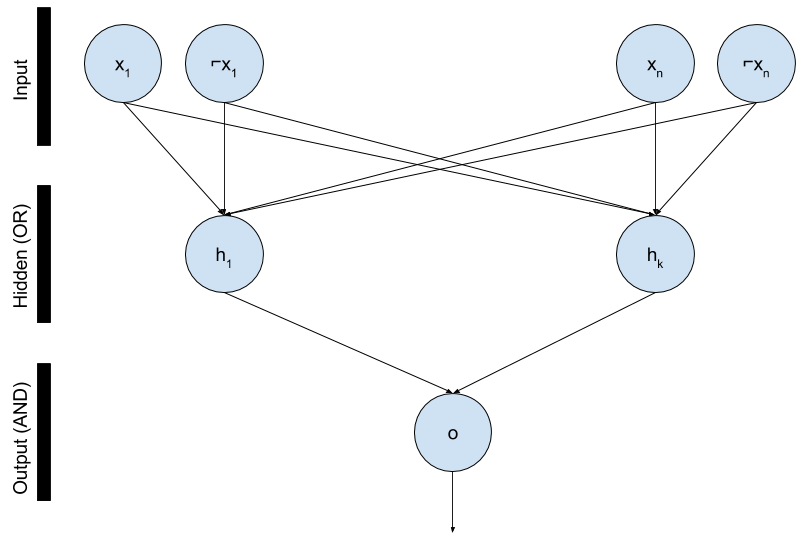
\includegraphics[width=\textwidth]{CNF-Network-Structure.png}
		\caption{Network Architecture for Learning CNF}
		\label{fig:cnf-network-structure}
	\end{minipage}
	\hfill
\end{figure}
\end{minipage}

\theoremstyle{definition}
\begin{definition} \label{def:cnf-network}
A \textbf{CNF-Network} is a three layer network where neurons in the hidden layer consist solely of Noisy-OR's and the output layer is a single Noisy-AND. 
\end{definition}

\theoremstyle{definition}
\begin{definition} \label{def:dnf-network}
A \textbf{DNF-Network} is a three layer network where neurons in the hidden layer consist solely of Noisy-AND's and the output layer is a single Noisy-OR. 
\end{definition}

\theoremstyle{definition}
\begin{definition} \label{def:lnfn}
A \textbf{LNF-Network} is a DNF or CNF Network
\end{definition}

Theorem \ref{thm:upper-bound-hidden-units} proves that a CNF or DNF Network should have a hidden layer size of $2^n$ to guarantee that the formulae can be learnt.

\begin{theorem}
Let T be the complete truth table for the boolean formula B. Let L be an LNFN, if L has $2^n$ hidden units then there always exists a set of weights for L which correctly classifies any assignment of truth values to atoms.
\label{thm:upper-bound-hidden-units}
\end{theorem}

A proof of Theorem \ref{thm:upper-bound-hidden-units} is given in Appendix \ref{apendix:proofs}. Theorem \ref{thm:upper-bound-hidden-units} provides justification for using $2^n$ hidden units, it guarantees that there at least exists an assignment of weights yielding a network that can correctly classify each item in the truth table.

\section{Noisy Gate Parametrisation} \label{sec:real-noisy-parametrisation}
The parametrisation of Noisy gates require weight clipping, an expensive operation. A new parametrisation is derived that implicitly clips the weights. Consider that $\epsilon \in (0, 1]$, therefore let $\epsilon_i = \sigma(w_i)$, these $w_i$'s can be trained without any clipping, after training the original $\epsilon_i$'s can be recovered.\\

Now these weights must be substituted into the Noisy activation. Consider the Noisy-OR activation.

\begin{align*}
a_{or}(X) &= 1 - \prod^p_{i=1}(\epsilon_i^{x_i})\\
&= 1 - \prod^p_{i=1}(\sigma(w_i)^{x_i})\\
&= 1 - \prod^p_{i=1}((\frac{1}{1 + e^{-w_i}})^{x_i})\\
&= 1 - \prod^p_{i=1}((1 + e^{-w_i})^{-x_i})\\
&= 1 - e^{\sum^p_{i=1} -x_i \cdot ln(1 + e^{-w_i})} \\
&Let\ w_i^{'} = ln(1 + e^{-w_i})\\
&= 1 - e^{-(W^{'} \cdot X)}
\end{align*}

From a similar derivation we get the activation for a Noisy-AND.

\begin{align*}
a_{and}(X) &= \prod_{p}^{i=1} (\epsilon_i^{1 - x_i})\\
&= \prod_{p}^{i=1} (\sigma(w_i)^{1 - x_i})\\
&= e^{\sum^p_{i=1} -(1 - x_i) \cdot ln(1 + e^{-w_i})}\\
&= e^{-(W^{'} \cdot (1 - X))}
\end{align*}

Concisely giving equations \ref{equ:real-noisy-and-activation}, \ref{equ:real-noisy-or-activation}

\begin{align}
a_{and}(X) &= e^{-(W^{'} \cdot (1 - X))} \label{equ:real-noisy-and-activation}\\
a_{or}(X)&= 1 - e^{-(W^{'} \cdot X)} \label{equ:real-noisy-or-activation}
\end{align}

The function taking $w_i$ to $w_i^{'}$ is the soft ReLU function which is performing a soft clipping on the $w_i$'s. 

\section{Training LNF Networks}
Using equations \ref{equ:real-noisy-or-activation} and \ref{equ:real-noisy-and-activation} for the Noisy-OR, Noisy-AND activations retrospectively allows LNFNs to be trained without the need to clip the weights.\\

Before these networks can be trained a number of choices must be made. These are outlined in the list below.

\begin{enumerate}
	\item \textit{Weight Initialization:} A method for initializing the weights must be derived. In the case of MLPNs it was shown that if initialization of weights is not carefully thought about as the number of neurons increases the learning conditions deteriorate \cite{glorot2010understanding}.
	\item \textit{Training Algorithm:} There exists a number of different algorithms for propagating gradients \cite{ruder2016overview}. One must be chosen based on the properties of these networks.
	\item \textit{Batch Size:} What size should each batch be when training these networks.
\end{enumerate}

\subsection{Weight Initialization}
Poor weight initialization leads to slower or poor convergence \cite{mishkin2015all}. Weight initialization algorithms can not be universally applied to different activations. A method derived for MLPNs was shown to be ineffective for networks using other activations \cite{he2015delving}.

\paragraph{Deriving a Distribution For The Weights}
Before a weight initialization algorithm can be derived good learning conditions must be identified. The function $e^{-z}$ squash a variable $z$ into the range $[0,1]$, Figure \ref{fig:activation-plot} shows a graph of this function.\\
\noindent
\begin{minipage}[t]{0.55\textwidth}
\vspace{0px}
At $z \geq 4$ the function $e^{-z}$ changes very little as it gets asymtoticly close to 0. This means that $e^{-z}$ suffers from what is known as saturation. If the method of initializing weights does not consider the inputs to a neuron then at a certain point the weighted sum of inputs will always be $\geq 4$ and thus the activation will always be constant. The sigmoid function suffered from this problem and one method of fixing it was careful initilizaton of the weights \cite{glorot2010understanding}. The approach here is to derive an initial weight distribution which keeps the variance and mean of neuron activations the same throughout the network \cite{kumar2017weight}. \\
\end{minipage}
\hspace{0.05\textwidth}
\begin{minipage}[t]{0.4\textwidth}
\vspace{0px}
\begin{figure}[H]
\vspace{0px}
    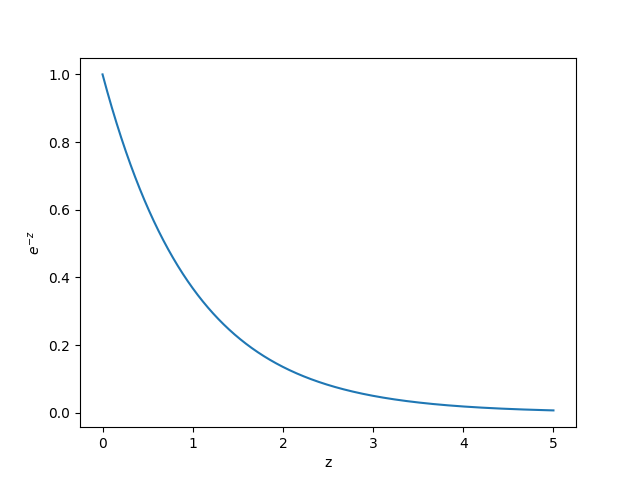
\includegraphics[width=\textwidth]{activation-plot.png}
    \caption{Plot of $e^{-z}$}
    \label{fig:activation-plot}
\end{figure}
\end{minipage}

As with previous approaches to solving this problem it will be assumed the inputs to the network are independent and weights are independent and identically distributed (i.i.d). It has previously been proved that these assumptions are enough to show the inputs to any layer are independent \cite{kumar2017weight}.\\

Ideally the output of each neuron would be varied for each training example, i.e. $y \sim U(0,1)$. Each training example $X = \{x_1, ..., x_n\}$ has each component $x_i \in (0,1]$, it will be assumed that $x_i \sim U(0,1)$. 

\noindent
\begin{minipage}[t]{0.55\textwidth}
\vspace{0px}
If the input vectors and output of each neuron are both distributed $U(0,1)$ then the input to any layer is distributed $U(0,1)$. Based on these facts it can be argued that the weight initialization is the same for both Noisy-OR and Noisy-AND, first recall the activations for Noisy neurons given in Figure \ref{fig:recall-noisy-activations}.\\
\end{minipage}
\hspace{0.05\textwidth}
\begin{minipage}[t]{0.4\textwidth}
\vspace{0px}
\begin{figure}[H]
\vspace{0px}
{\centering
$ \displaystyle
\begin{aligned}
a_{AND}(X) &= e^{-(w_1(1 - x_1) + ... + w_n(1 - x_n))}\\
a_{OR}(X) &= 1 - e^{-(w_1x_1 + ... + w_nx_n)}
\end{aligned}
$
\par}
\caption{Noisy Neuron Activations}
\label{fig:recall-noisy-activations}
\end{figure}
\end{minipage}

Consider a random variable $g$, if $g \sim U(0,1)$ then $1 - g \sim U(0,1)$ also holds. Consequently, if $x_i \sim U(0,1)$ then $1 - x_i ~ U(0,1)$, also $e^{-z} \sim U(0,1)$ then $1 - e^{-z} ~ U(0,1)$. It is therefore enough to consider $e^{-(w_1x_1 + ... + w_nx_n)}$ when deriving the initialization method for each $w_i$. Each $w_i = \log(1 + e^{w^{'}_i})$ (as derived in Section \ref{sec:real-noisy-parametrisation}) however for the purposes of this initialisation derivation this will be forgotten for now. Given that $y = e^{-z} ~ U(0,1)$, a first step is to determine the distribution of $z$.\\
\begin{theorem}
	If $y \sim U(0,1)$ and $y = e^{-z}$, then $z \sim exp(\lambda = 1)$
\end{theorem}
\begin{proof}
	Consider that $y = e^{-z}$ can be re written as $z = -\log(y)$. The Cumulative Distribution Function (CDF) will be derived for $z$.
	
	\begin{align*}
	F(z) &= P(Z < z)\\
	&= P(-\log(Y) < z)\\
	&= P(\frac{1}{Y} < e^{-z})\\
	&= P(Y \geq e^{-z})\\
	&= 1 - P(Y \leq e^{-z})\\
	&= 1 - \int_{0}^{e^{-z}} f(y) dy\\
	&= 1 - \int_{0}^{e^{-z}} 1 dy\\
	&= 1 - e^{-z}
	\end{align*}
	
	Therefore $F(z) = 1 - e^{-\lambda z}$ where $\lambda = 1$. So $z$ has the CDF of an exponential distribution. Consequently $z \sim exp(\lambda = 1)$
\end{proof}

The problem has now been reduced to find how $w_i$ is distributed given that $z \sim exp(\lambda = 1)$ and $x_i \sim U(0,1)$. The approach taken is to find $E[w_i]$ and $var(w_i)$.

\begin{align*}
E[z] &= E[w_1x_1 + \cdot \cdot \cdot + w_nx_n]\\
&= E[w_1x_1] + \cdot \cdot \cdot + E[w_nx_n]\ (independence)\\
&= E[w_1]E[x_1] + \cdot \cdot \cdot + E[w_n]E[x_n]\\
&= n \cdot E[w_i]E[x_i]\ (i.i.d)\\
&= n \cdot E[w_i] \cdot \frac{1}{2}\\
1 &= \frac{n}{2} \cdot E[w_i]\\
E[w_i] &= \frac{2}{n}
\end{align*}

\begin{align*}
var(z) &= var(w_1x_1 + \cdot \cdot \cdot + w_nx_n)\\
&= var(w_1x_1) + \cdot \cdot \cdot + car(w_nx_n)\\
\end{align*}

\begin{align*}
var(w_ix_i) &= (E[w_i])^2var(x_i) + (E[x_i])^2var(w_i) + var(w_i)var(x_i)\\
&= \frac{4}{n^2} \cdot \frac{1}{2} + \frac{1}{4} \cdot var(w_i) + var(w_i) \cdot \frac{1}{12}\\
&= \frac{1}{3 n^2} + \frac{1}{3}var(w_i)
\end{align*}

Consequently the variance can be found by the following

\begin{align*}
1 &= n \cdot \big[\frac{1}{3 n^2} + \frac{1}{3}var(w_i)\big]\\
3 &= \frac{1}{n} + n \cdot var(w_i)\\
3n &= n^2 var(w_i)\\
var(w_i) &= \frac{3}{n}
\end{align*}

From the above arguments $E[w_i] = \frac{2}{n}$ and $var(w_i) = \frac{3}{n}$. These values need to be fitted to a distribution that weights can be sampled from. Based on our initial assumptions this distribution must also generate values in the interval $[0, \infty]$. There exists a number of different distributions which satisfy this constraint. The distribution which had the best results was log-normal \cite{balakrishnan2006continuous}, for brevity only its derivation is included.

\paragraph{Fitting To Log Normal}

A Log-Normal distribution has two parameters $\mu$ and $\sigma^2$, by the definition of Log-Normal $E[w_i] = \frac{2}{n} = e^{\mu + \frac{\sigma^2}{2}}$ and $var(w_i) = \frac{3}{n} = \big[e^{\sigma^2} - 1\big] \cdot e^{2\mu + \sigma^2}$. Consequently

\begin{align*}
\frac{2}{n} &= e^{\mu + \frac{\sigma^2}{2}}\\
\log(\frac{2}{n}) &= \mu + \frac{\sigma^2}{2}\\
\log(\frac{4}{n^2}) &= 2\mu + \sigma^2
\end{align*}

From here this can be substituted into the other formula to give

\begin{align*}
\frac{3}{n} &= \big[e^{\sigma^2} - 1\big] \cdot e^{2\mu + \sigma^2}\\
&= \big[e^{\sigma^2} - 1\big] \cdot e^{\log(\frac{4}{n^2})}\\
&= \big[e^{\sigma^2} - 1\big] \cdot \frac{4}{n^2}\\
3n &= 4 \cdot e^{\sigma^2} - 4\\
\frac{3n + 4}{4} &= e^{\sigma^2}\\
\sigma^2 = \log \frac{3n + 4}{4}
\end{align*}

Finally this substituted back gives the mean

\begin{align*}
\log(\frac{4}{n^2}) &= 2\mu + \log \frac{3n + 4}{4}\\
2\mu &= \log(\frac{4}{n^2}) - \log \frac{3n + 4}{4}\\
\mu &= \frac{1}{2} \cdot \log \frac{16}{n^2(3n + 4)}
\end{align*}

Giving the parameters for the log normal distribution below
\begin{align}
\sigma^2 &= \log \frac{3n + 4}{4}\\
\mu &= \frac{1}{2} \cdot \log \frac{16}{n^2(3n + 4)}
\end{align}


\noindent
\begin{minipage}[t]{0.48\textwidth}
\vspace{0px}
\paragraph{Weight Initialization Algorithm}
Figure \ref{alg:lnn-initlization} gives the algorithm for initializing weights for Noisy neurons. Each weight that is sampled from the Log Normal distribution. Recall $w = f(w^{'})$ where $w^{'}$ can be any real value, consequently to obtain the initial weights each $w$ must be inversely transformed using $f^{-1}$.
\end{minipage}
\hspace{0.05\textwidth}
\begin{minipage}[t]{0.47\textwidth}
\vspace{0px}
\begin{figure}[H]
	\begin{lstlisting}[mathescape=true]
function constructWeights(size):
$w_i \sim LN$ (for i = 0 to size)
return $f^{-1}(\{w_0, ...\})$
\end{lstlisting}
	\caption{Weight Initialization Algorithm for LNNs}
	\label{alg:lnn-initlization}
\end{figure}
\end{minipage}

\subsection{Training Algorithm}
The ADAM Optimizer \cite{kingma2014adam} is the learning algorithm which will be used. For the convenience of an adaptive learning rate and because it has been shown that networks of this form yield a sparse representation, which the ADAM algorithm works well with.

\subsection{Batch Size}
The batch size will be fixed to one. Experimental results from training an LNFN with a batch size of 1 converged faster. 

\section{LNF Network Performance}
Preliminary testing showed that LNFN's are able to learn good classifiers on boolean gates, i.e. NOT, AND, NOR, NAND, XOR and Implies. How do LNFNs perform against standard MLPNs which are known to be universal function approximators? Two different MLPNs will be used as a benchmark

\begin{enumerate}
	\item One will have the same configuration as the LNFNs, i.e. $2^n$ hidden neurons. \label{lnfn-peformance:mlpn-arch-1}
	\item The other has two hidden layers, both with N neurons.
\end{enumerate}

The testing will consist of selecting 5 random boolean expressions for $2 \leq n \leq 9$ and training each network 5 times, each with random initial conditions. Figure \ref{fig:peformance-comparason-all} shows a comparison between all 4 of the networks and Figure \ref{fig:peformance-comparason-cnfdnf} shows just the LNFN's.

\begin{figure}[H]
  \centering
  \begin{minipage}[b]{0.45\textwidth}
    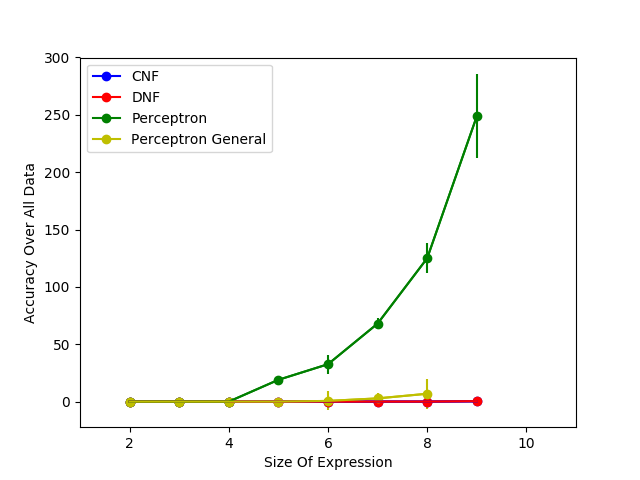
\includegraphics[width=\textwidth]{All-Peformance-Comparason.png}
    \caption{}
    \label{fig:peformance-comparason-all}
  \end{minipage}
  \begin{minipage}[b]{0.45\textwidth}
    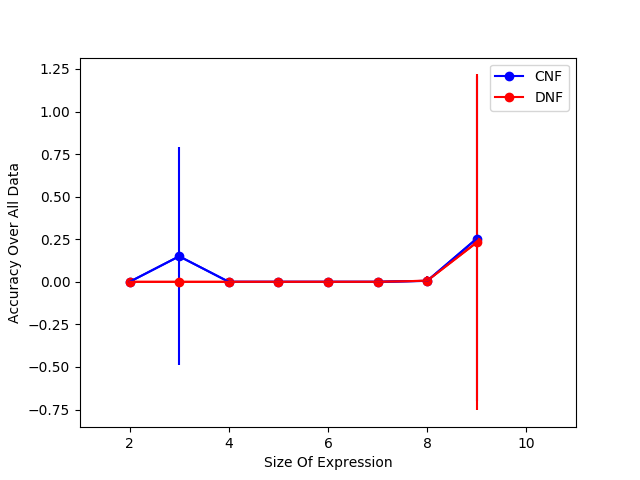
\includegraphics[width=\textwidth]{CNFvsDNF.png}
    \caption{}
    \label{fig:peformance-comparason-cnfdnf}
  \end{minipage}
  \hfill
\end{figure}

Figure \ref{fig:peformance-comparason-all} show that the LNFNs have statistically equivalent performance to one of the configurations of MLPNs and the other Perceptron network with $2^n$ hidden neurons has poor performance. Figure \ref{fig:peformance-comparason-cnfdnf} shows that CNF and DNF networks have statistically equivalent performance. 

\section{LNF Network Generalization} \label{sec:lnfn-generalization}
These networks are able to perform as well as standard perceptron networks but so far they have been trained on a complete data set. In practice this will almost never be the case. Standard ANN's are widely used because of their ability to generalize. Here the generalization capability of LNFNs will be tested against that of MLPNs

\begin{figure}[H]
	\centering
	\begin{minipage}[t]{0.6\textwidth}
		\vspace{0px}
		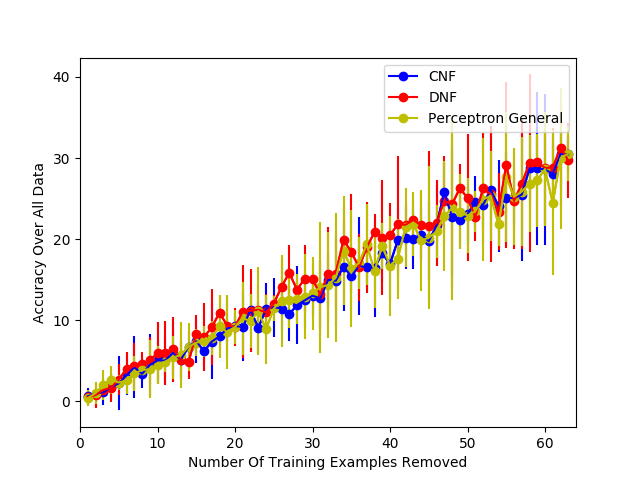
\includegraphics[width=\textwidth]{6-generalization.png}
		\caption{}
		\label{fig:generalization-peformance-6}
	\end{minipage}
	\begin{minipage}[t]{0.39\textwidth}
	\vspace{0px}
		Figure \ref{fig:generalization-peformance-6} shows a comparison between the generalization ability of CNF, DNF and Perceptron networks. The graph shows the performance over all training data when successively removing elements from the training set. It demonstrates that the CNF and DNF networks generalize as well as the perceptron networks when trained over boolean problems with 6 inputs, this trend continues as n increases up to 9. Training LNFNs on boolean problems with more than 9 inputs is to expensive.		
	\end{minipage}
	\hfill
\end{figure}

\section{LNF Network Rule Extraction} \label{sec:lnfn-rule-extraction}
Consider the weights for a logical neuron $W = \{w_1, ..., w_n\}$. These can be converted to $\epsilon_i = \sigma(w_i)$ where $\epsilon_i \in [0, 1]$ and represents the relevance input $x_i$ has on the neurons output.\\

To extract boolean rules from the network it must be possible to interpret each neuron as a logical function acting on a subset of its inputs. For this to be the case, at the conclusion of training either $\epsilon_i \approxeq 1$ or $\epsilon_i \approxeq 0$ needs to be true. If each $\epsilon_i$ is either 1 or 0 then the neuron is a logical function of the inputs which have corresponding $\epsilon \approxeq 0$. Conjecture \ref{conj:lnfn-approach-binary} is the foundation of the following rule extraction algorithm, it was derived from experimental evidence by training LNFNs over complete truth tables and inspecting the weights. Ideally Conjecture \ref{conj:lnfn-approach-binary} would be proved, but that is out of scope for this report.

\begin{conjecture}
	For an LNFN network trained on a binary classification problem with boolean inputs as the loss approaches 0  (i.e. the correct CNF or DNF has been found) the weights $\{ w_1, ..., w_n \}$ approach $\infty$ or $-\infty$. Consequently each $\epsilon_i = \sigma(w_i)$ (where $\sigma(\cdot)$ is the sigmoid function) approaches 0 or 1.
	\label{conj:lnfn-approach-binary}
\end{conjecture}

\noindent
\begin{minipage}[t]{0.3\textwidth}
\vspace{0px}
The Algorithm displayed in figure \ref{alg:rule-extraction} extracts rules from CNFNs. It takes the output weights (ow) and hidden weights (hw) as input and outputs the a boolean expression. A similar algorithm can be derived for DNFNs, it is omitted but can be obtained by simply switching the logical operations around. In practice many clauses in the extracted expression contain redundant terms, such as clauses that are a tautology or a duplicate of another.\\
\end{minipage}
\hspace{0.05\textwidth}
\begin{minipage}[t]{0.65\textwidth}
\vspace{0px}
\begin{figure}[H]
	\begin{lstlisting}[mathescape=true]
atoms = $\{ x_1, ... x_n, \lnot x_1, ..., \lnot x_n, \}$
	
function extractRulesCNFN(ow, hw)
  ow $= \sigma($ow$)$
  hw $= \sigma($hw$)$
  relvHidden = [hw[i] where ow[i] := 0]

  and=And([])
    for weights in relvHidden
      or=Or([atoms[i] where weights[i]:=0])
      and.add(or)
		
  return and
	\end{lstlisting}
	\caption{Rule Extraction Algorithm (for CNFN)}
	\label{alg:rule-extraction}
\end{figure}
\end{minipage}

How does training over incomplete truth tables effect the generalization of extracted rules and what factors could influence this?\\

Consider $B$ to be the set of all boolean problems with $n$ inputs. What is the cardinality of $B$? There are $2^n$ rows in the truth table and $2^{2^n}$ ways to assign true/false values to these rows, each way corresponding to a different boolean function. Consequently $|B| = 2^{2^n}$. Consider some $b \in B$ represented by $2^n$ rows of a truth table, removing one row from the training data means there are now two possible functions that could be learnt, one where the removed row corresponds to true and the other to false. As more rows are removed this problem is compounded. If $m$ rows are taken then there are $2^m$ possible functions that $b$ could represent.\\

To test the generalization of the CNFN and DNFN rule sets LNFNs will be trained over a randomly generated boolean problem with 4 inputs. The training set will reduce in size one by one and the extracted rules will be evaluated over the entire tuth table. For each training set size the experiment will be repeated 30 times. Figures \ref{fig:cnf-descrete-generalizatiion} \& \ref{fig:dnf-descrete-generalizatiion} shows the number of examples removed from the training set on the x axis. The y axis shows the number of incorrectly classified instances over the entire dataset. These experiments show that when no examples are removed then the rules can achieve a perfect accuracy. As instances are removed from the training set the rules are able to generalise on average. 

\begin{figure}[H]
	\centering
	\begin{minipage}[b]{0.45\textwidth}
		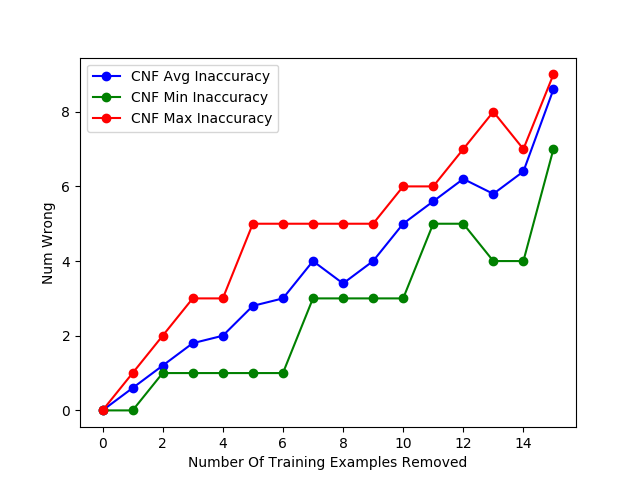
\includegraphics[width=\textwidth]{cnf-descrete-generalization.png}
		\caption{CNFN trained using an incomplete truth table}
		\label{fig:cnf-descrete-generalizatiion}
	\end{minipage}
	\begin{minipage}[b]{0.45\textwidth}
		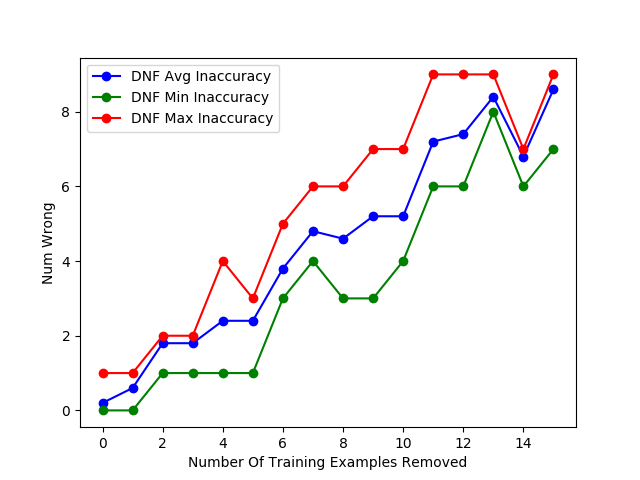
\includegraphics[width=\textwidth]{dnf-descrete-generalization.png}
		\caption{DNFN trained using an incomplete truth table}
		\label{fig:dnf-descrete-generalizatiion}
	\end{minipage}
	\hfill
\end{figure}

When constructing a CNF from a truth table (See Section \ref{subsec:construct-cnfdnf}) only the rows corresponding to false are considered. Is it then possible that by only removing rows which correspond to false a CNFN can learn rules which achieve a perfect accuracy. Figure \ref{fig:cnf-descrete-generalizatiion-partial} represents this situation.

\begin{figure}[H]
	\centering
	\begin{minipage}[b]{0.45\textwidth}
		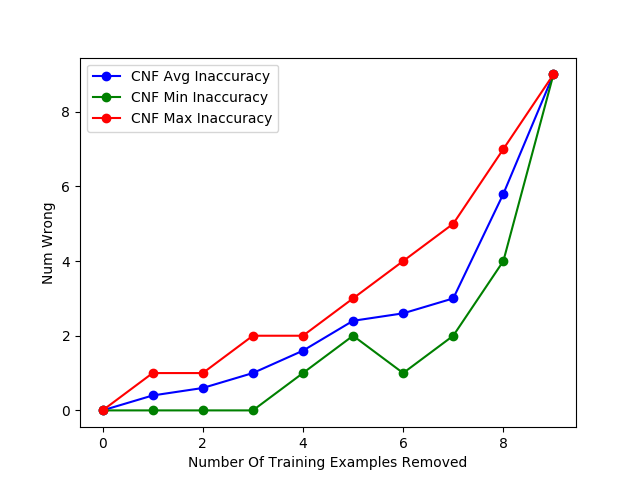
\includegraphics[width=\textwidth]{cnf-descrete-generalization-partial.png}
		\caption{CNFN trained using an incomplete truth table, only rows corresponding to false are removed}
		\label{fig:cnf-descrete-generalizatiion-partial}
	\end{minipage}
	\begin{minipage}[b]{0.45\textwidth}
		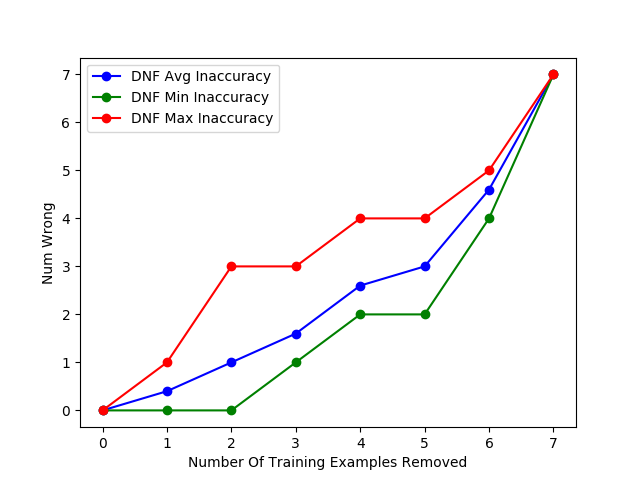
\includegraphics[width=\textwidth]{dnf-descrete-generalization-partial.png}
		\caption{DNFN trained using an incomplete truth table, only rows corresponding to true are removed}
		\label{fig:dnf-descrete-generalizatiion-partial}
	\end{minipage}
	\hfill
\end{figure}

Figures \ref{fig:cnf-descrete-generalizatiion-partial} \& \ref{fig:dnf-descrete-generalizatiion-partial} show CNFNs and DNFNs trained over partial data retrospectively. In the case of CNFNs only entries corresponding to true in the truth table are removed and for the DNFNs only false entries. These graphs show that careful removal of each training example does not result in rules that perform better. These results indicate that the generalization of extracted rule sets depends on the initial condtions rather than what examples are removed.

\section{Summary}
In this chapter a method for training LNFNs was derived. LNFNs where shown to have statistically equivalent performance and generalization to MLPNs. Finally it was shown that rules can be extracted from LNFNs and that these rule sets where able to generalise.

\chapter{Expanding the Problem Domain of Logical Normal Form Networks} \label{C:investigation-of-lnfns}
The LNFNs presented in Chapter \ref{C:foundation-of-lnfns} have only been shown to be applicable when learning boolean truth tables. This chapter investigates extending LNFNs to support multi class classification problems and continuous feature spaces.

\section{Multi-class Classification}
Extending an ANN to support multi class classification is achieved by adding more output neurons, one for each class. The value output neuron $i$ can be considered the probability of class $i$. The networks output is now a vector representing the class distribution. \\

For example if given a problem with 3 classes then $\{1,0,0\}$, $\{0,1,0\}$ and $\{0,0,1\}$ represent class 1, 2 and 3 retrospectively. The LNFN would have 3 output neurons, each representing a bit in the output vector. During the training process if the true class of an example was 1 then the desired output vector would be $\{1,0,0\}$. This process of converting a categorical variable to a binary string is known as \textbf{One-Hot Encoding}

\begin{definition}
	An LNFN to solve a $k$ class classification problem is unchanged apart from the number of output neurons which is $k$.
\end{definition}

\subsection{Application to Lenses Problem}
The Lenses problem \cite{Lichman:2013} is multi class and contains a natural rule system making it an ideal problem for evaluating LNFNs. The goal is to determine whether (if any) contact lenses should be fitted to the patient. There are 3 classes, fit soft, fit hard and do not fit any. Each example has four features, three are binary and one categorical (of size 3). Applying One-Hot encoding to the categorical variable yields a set of instances each with length 6.\\

The LNFN will be evaluated against an MLPN with a two layer structure where the layer width are $2 \cdot n$ and $n$ retrospectively.\\

The performance of the two classifiers will be compared using Leave-One-Out Cross-Validation. The structure of the MLPN differs in the number of hidden layers/units, there are two hidden layers, one with $2 \cdot n$ hidden units and the other with $n$

\begin{table}[H]
	\begin{center}
		\begin{tabular}{| c | c | c |}
			\hline
			& Error Rate & Error Rate CI (95\%) \\
			\hline
			\hline
			CNF Net & 0.0122 & (0.0000, 0.0417) \\
			\hline
			DNF Net & 0.0104 & (0.0000, 0.0417) \\
			\hline
			MLPN Net & 0.0000 & (0.0000, 0.0000) \\
			\hline
		\end{tabular}
	\end{center}
	\caption{Network Performance On Lenses Problem}
	\label{tab:lenses-peformance-comp}
\end{table}

Table \ref{tab:lenses-peformance-comp} demonstrates that the CNF \& DNF Networks perform comparably to an MLPN as the confidence intervals for the errors overlap.\\ 

Now that the LNFN network has three output neurons it should be possible to extract three rules describing each of the classes. Consider that each problem instance is of the following form $\{a, b, c, d, e, f\}$ where $a,b,c,d,e,f$ are all atoms. $f$ refers to the \textit{tear production rate} being normal or reduced if $f = False$ or $True$ retrospectively. Giving a description of the other atoms is not beneficial as they refer to medical terms which are unimportant.\\

The list of rules in Figure \ref{fig:lenses-cnfn-rules} have been extracted from a CNFN after being trained over the complete Lenses data set. These rules contain redundancies which could be filtered out automatically.

\begin{figure}[H]
	\begin{itemize}
		\item \text{Class 1:} $(a \lor \lnot d) \land (e \lor \lnot f) \land (\lnot ( \lnot f )) \land (\lnot (\lnot e \lor \lnot f)) \land (\lnot(e \lor \lnot f))$
		\item \text{Class 2:} $(a \lor b \lor d \lor e \lor \lnot c) \land (\lnot(e \lor \lnot f)) \land (\lnot(e \lor \lnot f)) \land (\lnot(e \lor \lnot f))$
		\item \text{Class 3:} $(c \lor e \lor \lnot b \lor \lnot f) \land (e \lor \lnot d \lor \lnot f) \land (d \lor \lnot e \lor \lnot f) \land (b \lor c \lor \lnot a \lor \lnot f) \land (b \lor c \lor d \lor e \lor \lnot a \lor \lnot d \lor \lnot e \lor \lnot f) $
	\end{itemize}
	\caption{CNF rules extracted from CNFN}
	\label{fig:lenses-cnfn-rules}
\end{figure}


Immediately it is possible to find useful information about this problem that was not obvious before. For example $\lnot f = True \implies $ Class 3, or \textit{if the tear reduction rate is reduced then do not fit contact lenses}. Alternatively DNF rules could be constructed using a DNFN, this possibility is demonstrated in the following three rules.

\begin{itemize}
	\item \text{Class 1:} $(a \land d \land e \land f \land \lnot b \land \lnot c) \lor (a \land d \land e \land f \land \lnot b \land \lnot c) \lor (e \land f \land \lnot d)$
	\item \text{Class 2:} $(f \land \lnot c \land \lnot d \land \lnot e) \lor (d \land f \land \lnot e)$
	\item \text{Class 3:} $(e \land e \land \lnot a) \lor (c \land f \land \lnot a \land \lnot b \land \lnot d \land \lnot e) \lor (\lnot f) \lor (\lnot f)$
\end{itemize}

The formulae extracted from the DNFN confirm previous knowledge obtained from the CNFN, namely $\lnot f = True \implies $ Class 3. Table \ref{tab:lenses-rule-peformance-comp} demonstrates the performance of extracted rules over the Lenses dataset. The confidence intervals of networks and rule sets overlap so there is no statistically significant difference between the network and rule set in terms of their accuracy on the data.

\begin{table}[H]
	\begin{center}
		\begin{tabular}{| c | c | c |}
			\hline
			& Rule Error Rate & Rule Error Rate CI (95\%) \\
			\hline
			\hline
			CNF Rules & 0.0122 & (0.0000, 0.0417) \\
			\hline
			DNF Rules & 0.0156 & (0.0000, 0.0417) \\
			\hline
		\end{tabular}
	\end{center}
	\caption{}
	\label{tab:lenses-rule-peformance-comp}
\end{table}

The results shown thus far demonstrate that LNFNs can be applied to boolean multi class classification problems.

\section{Features with Continuous Domains}
It is possible for the inputs to a Noisy Neuron to be in the range $[0,1]$, but when does it make sense to do so? And what do these continuous features mean? The inputs can be thought of as being the probability that the feature is present. In the discrete case either the input is there (a 1) or not (a 0). Then in the continuous case each input feature is thought of as a probability.\\

How about the case where the feature range is not confined to $[0,1]$. An option is to normalise the feature spaces, forcing them into a format compatible with LNFNs. The problem then comes down to meaning. Is possible to think of these normalised features as a probability? Consider an arbitrary (un-normalised) feature $f$. Assume $f \in [f_{min}, f_{max}]$ then the larger the normalised feature $f_N$ the closer its true value is to $f_{max}$. Similarly if $\lnot f_N = 1 - f_N$ is large then the true value is closer to $f_{min}$. $f_N$ could then be the probability of sampling a $v \sim U(f_{min}, f_{max})$ that is less than $f$. This is certainly not the only meaning normalised features could have, it is simply an example.\\

Another consideration to make is, how can trained LNFN models be interpreted if the features are continuous? When the weights are binary then a Noisy neuron can be considered as a logical gate of its inputs with $\epsilon \approxeq 0$. The weights in a trained LNFN do not converge to 0 or 1 when the input features are continuous so a more general method to interpret LNFNs is needed.

\paragraph{Influence Model}
One potential way to interpret LNFNs would be to compute the influence each input feature has on the output neurons, this is defined to be an \textbf{Influence Model}.  The weights for a Noisy neuron directly correspond to the influence each input has on the neuron's output. Consequently it is a trivial task to find an Influence Model for describing how each input feature affects the hidden layer outputs, this is just the weights of each hidden neuron. Consider Figure \ref{fig:network-example}  and the problem computing an Influnce Model describing the influence each $x_i$ has on the output of some $o_j$.

\begin{figure}[H]
	\centering
	\begin{minipage}[t]{0.5\textwidth}
		\vspace{0px}
		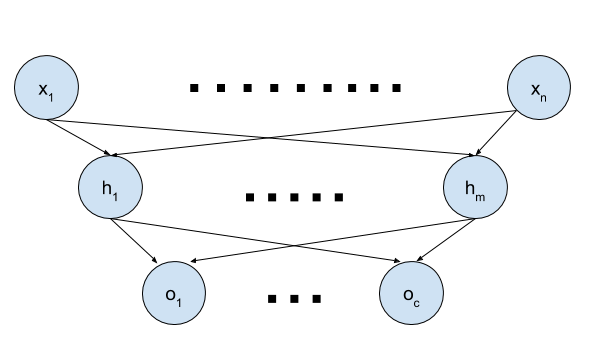
\includegraphics[width=\textwidth]{NetworkExample.png}
		\caption{Example Network}
		\label{fig:network-example}
	\end{minipage}
	\hspace{1px}
	\begin{minipage}[t]{0.45\textwidth}
		\vspace{2px}
		 In the following computations $\epsilon_i^{h_j}$ is the ith $\epsilon$ for neuron $h_j$. Assume all activations are Noisy-OR's, then the activation of $o_j$ is $1 - \prod^m_{k=1} (\epsilon_k^{o_j})^{h_k}$ and the activation of some $h_k$ is $1 - \prod^n_{b=1} (\epsilon_b^{h_k})^{x_b}$. The aim is therefore to find an $(\epsilon^{'}_i)$ that stasfies Equation \ref{equ:interpetation-across-layers}.
	
		\begin{align}
			(\epsilon^{'}_i)^{x_i} = \prod_{k = 1}^{m} (\epsilon^{o_j}_k)^{\prod_{b = 1}^{n} (\epsilon^{h_k}_b)^{x_b}}
			\label{equ:interpetation-across-layers}
		\end{align}
	\end{minipage}
	\hfill
\end{figure}

This new $\epsilon^{'}_i$ is dependent on all the other $x$'s, not just the $x_i$ of interest. Consequently there is not an obvious solution to computing Influence Model for LNFNs.

\paragraph{Partial Influence Models}
While it is not obvious how to compute an Influence Model describing a LNFN entirely it is trivial to compute one describing the influence between input features and the hidden layer output. Using this Partial Influence Model can describe the the hidden neurons in terms of the input features. The weights belonging to each output neuron could then be used to find the most important hidden neurons.

\paragraph{Continuous Rules}
Another way to interpret LNFNs in a continuous domain is to extract continuous rules. A threshold will be set, any input with a weight below the threshold will be considered important. Consequently each neuron will be considered a function of its inputs that have corosopnding weight less than or equal to a given threshold $t$. The same rule extraction algorithm (given in Figure \ref{alg:rule-extraction}) can therefore be used in both the discrete and continuous case if line 6 is adjusted to \textit{relvHidden = [hw[i] where ow[i] $\leq t$]}. The weights of all features will be truncated to 0 as if the weights where kept then it is essentially still an LNN with some connections removed. The continuous rules can be applied by using the Noisy activations with each $\epsilon \approxeq 0$. A potential issue with this method is that the less important features are removed after the threshold is applied, this might result in more incorrect classifications by the rules. A smaller threshold will lead to simpler rules with perhaps a higher error rate where as a larger threshold will give more complex rules with a possibly higher accuracy. This process also discards the true $\epsilon$'s which could potentially effect the accuracy of the rules.

\subsection{Application To Iris Problem}


The Iris data set \cite{Lichman:2013} is the problem of classifying a plant as one of three classes. Each example consists of four features, all are measurements taken from the plant. All features are in centimetres and not confined to the range $[0, 1]$. Table \ref{tab:iris-network-peformance-comp} gives the results of training the Normalised Iris problem on LNF networks. The results show that while the performance can vary a lot it is possible for both the CNF and DNF networks to obtain 100\% accuracy.

\begin{table}[H]
	\begin{center}
		\begin{tabular}{| c | c | c |}
			\hline
			& Error Rate & Error Rate CI (95\%) \\
			\hline
			\hline
			CNF Network & 0.027 & (0.000, 0.111) \\
			\hline
			DNF Network & 0.066 & (0.000, 0.156) \\
			\hline
		\end{tabular}
	\end{center}
	\caption{LNFN performance on an Iris problem testing set}
	\label{tab:iris-network-peformance-comp}
\end{table}

If attempting to interpret these models meaning must be assigned to each of the normalised features. Informally, an atom is "truer" if the un-normalised feature is larger and "falser" if its smaller. A NOT operation inverts this property. Table \ref{tab:iris-rule-peformance-comp} shows the performance of extracted continuous rules on a testing set. These performance statistics provide evidence that continuous rules have poor performance.

\begin{table}[H]
	\begin{center}
		\begin{tabular}{| c | c | c |}
			\hline
			& Error Rate & Error Rate CI (95\%) \\
			\hline
			\hline
			CNF Rules & 0.439 & (0.156, 0.867) \\
			\hline
			DNF Rules & 0.323 & (0.156, 0.511) \\
			\hline
		\end{tabular}
	\end{center}
	\caption{Performance of rules extracted from LNFN on an Iris problem testing set}
	\label{tab:iris-rule-peformance-comp}
\end{table}


\noindent
\begin{minipage}[t]{0.5\textwidth}
\vspace{0px}
The question remaining is, how do these rules contribute to interpreting the LNFN model. Figure \ref{fig:raw-iris-rules} shows raw continuous rules extracted from a DNFN. Features $\{a,b,c,d\}$ correspond to preferring larger values of $\{$ sepal length, sepal width, petal length, petal width $\}$. On the other hand $e = \lnot a, f = \lnot b, g = \lnot c, h = \lnot d$.\\

The list in Figure \ref{fig:iris-rules} shows some conclusions about the classes which can be drawn from the raw continuous rules. Having a small petal width and length mean the class is more likely to be \textit{Iris Setosa}. \\
\end{minipage}
\hspace{0.05\textwidth}
\begin{minipage}[t]{0.45\textwidth}
\vspace{0px}
\begin{figure}[H]
\begin{enumerate}
\item \textit{Iris Setosa:} $(g \land h) \lor (g \land h) \lor (g \land h) \lor (g \land h)$
\item \textit{Iris Versicolour:} $(c \land e \land f \land h) \lor (c \land f \land h) \lor (c \land f \land h) \lor (c \land e \land f \land h) \lor (c \land f \land h)$
\item \textit{Iris Virginica:} $(c \land d \land f) \lor (c \land d \land f) \lor (d \land f) \lor (c \land d \land f) \lor (c \land d \land f) \lor (c) \lor (c \land d \land f)$
\end{enumerate}
\caption{Raw continuous rules extracted from a DNFN, with a threshold of $0.5$}
\label{fig:raw-iris-rules}
\end{figure}
\end{minipage}

Alternatively having a larger petal width means the instance is more likely to be \textit{Iris Versicolour} or \textit{Iris Virginica}.

\begin{figure}[H]
	\centering

	\begin{minipage}[p]{0.51\textwidth}
	 Finally the \textit{Iris Versicolour} rule is more complicated and seems contradictory. If the instance has a small petal width and length but also has a large petal width or length.
	 \begin{figure}[H]
	 	\begin{enumerate}
	 		\item \textit{Iris Setosa: } Smaller \textbf{petal width} $\land$ Smaller \textbf{petal length}
	 		\item \textit{Iris Versicolour: } Larger \textbf{petal length} $\land$ Smaller \textbf{petal width} $\land$ Smaller \textbf{sepal width}
	 		\item \textit{Iris Virginica: } Larger \textbf{petal length} $\lor$ (Large \textbf{petal width} $\land$ Small \textbf{sepal width})
	 	\end{enumerate}
 		\caption{Rules representing the iris problem, extracted from a CNFN}
 		\label{fig:iris-rules}
	 \end{figure}
	\end{minipage}
	\hspace{4px}
	\begin{minipage}[p]{0.45\textwidth}
		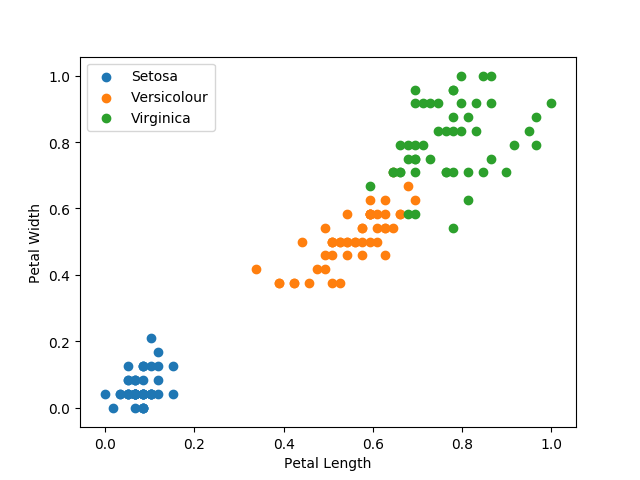
\includegraphics[width=\textwidth]{IrisData(petal(length-vs-width)).png}
		\caption{Scatter plot of Iris dataset, showing the petal length on the x-axis and petal width on the y-axis}
		\label{fig:iris-data-petal-length-vs-width}
	\end{minipage}
	\hfill
\end{figure}

Figure \ref{fig:iris-data-petal-length-vs-width} plots the petal width and length features against each other, demonstrating the conclusions drawn make sense.\\

This section has shown that LNFNs can be applied to any problem with continuous features by normalisation. This operation creates an additional problem, namely it becomes difficult to interpret what the normalised features mean. Future work into LNNs might aim to develop a better way to convert feature domains to probabilities.

\section{Summary}
This chapter has demonstrated that LNFNs can be applied to more than just learning boolean truth tables. They have been shown to achieve good accuracy on multi class classification problems, with and without discrete input features. A number of methods for interpreting LNFNs applied to continuous feature spaces. These methods where then shown to provide useful insights into the Iris dataset.\\

In the context of the Lenses problem it was possible to extract boolean rules from the LNFNs which had a statistically equivalent performance to the networks. These rules also provided incite into the problem which was not obvious from the data. The LNFNs where able to achieve a low error rate (sometimes 0\%) on the Iris data set. It was possible to extract useful information from the trained models which highlighted the most important features when making classifications. The experiments with the Iris problem also revealed limitations of LNNs

\chapter{Logical Neural Networks} \label{C:lnn}
This chapter discusses development of Logical Neural Networks as a generalization of LNFNs. There are two key issues with LNFNs. Firstly the number of hidden units becomes infeasible as the amount of inputs increases. Secondly if the problem size is small enough and the network can be trained the volume of hidden neurons allows for the possibility to memorise the input data. Using what has been learnt about LNFNs the class of Logical Neural Networks (LNNs) can be defined.

\begin{definition}
	A \text{Logical Neural Network} is an ANN where each neuron has a noisy activation.
\end{definition}

LNNs have a more flexible structure, allowing for deeper networks and hidden layers with a variable number of neurons. The current LNN model has been shown to have poor performance when compared to a Multi-Layer Perceptron Network \cite{LearningLogicalActivations}. An LNN, consisting of Noisy-OR hidden units and Noisy-AND outputs, was shown to perform worse than an MLPN. There are two key issues caused by removing the restrictions imposed by the LNFN definition (Definition \ref{def:lnfn}) which must be addressed 

\begin{enumerate}
	\item Noisy neurons do not have the capacity to consider the presence of the negation of an input. This was a problem for LNFNs as well, however given that only the negations of atoms need to be considered to learn a CNF or DNF it was easily fixed by presenting the network with each atom and its negation. The problem can not be solved so easily for LNNs. A boolean formula can not always be represented by only AND and OR gate, i.e the set of operations $\{AND, OR\}$ is not functionally complete. 
	
	\item Another problem faced by LLNs that are not restricted to be ether a CNFN or DNFN is that the structure of the network will have a higher impact on whether the problem can be learnt. 
\end{enumerate}

Resolving Issue 1 involves making our operation set functionally complete, this requires the $NOT$ operation. There are two ways to include the $NOT$ operation in the LNNs, one is to simply augment the inputs to each layer appending so it receives the input and its negation. Another is to derive a parametrisation of Noisy gates which can learn to negate inputs. However both these have no way to enforce mutual exclusivity between an input and its negation.

\section{Modified Logical Neural Network} \label{sec:modified-lnn}
\subsection{Connections Between Layers \& Parameters}
Figure \ref{fig:modified-lnn-structure} provides a new structure for the connections between the lectures.

\begin{figure}[H]
	\centering
	\begin{minipage}[b]{0.9\textwidth}
		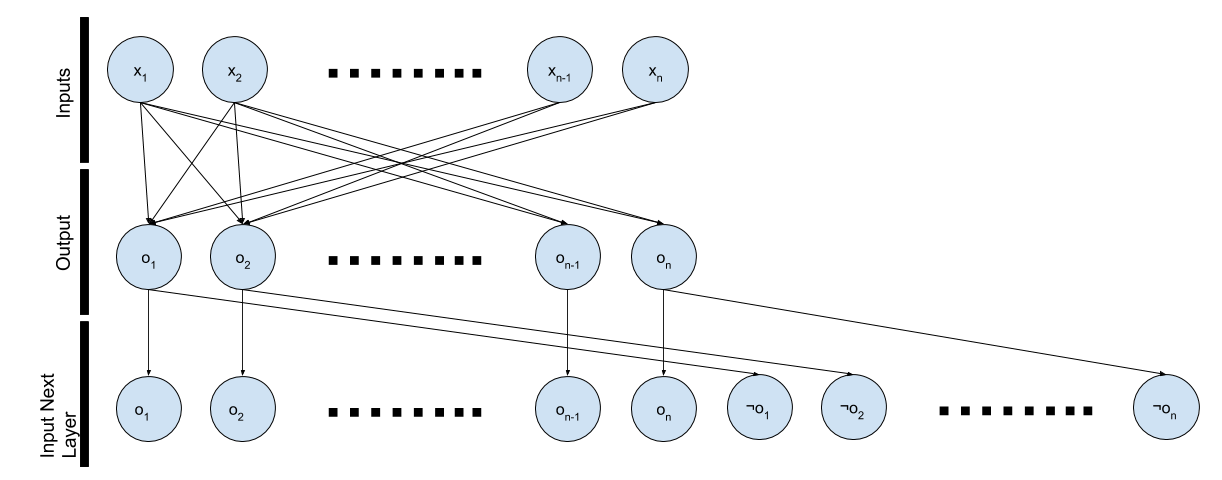
\includegraphics[width=\textwidth]{Modified-LNN-Structure.png}
		\caption{}
		\label{fig:modified-lnn-structure}
	\end{minipage}
	\hfill
\end{figure}

Figure \ref{fig:modified-lnn-structure} shows the new LNN structure which includes an implicit NOT operation. The input to each layer consists of the true output of the previous plus the negated output from the last layer. If a layer has 20 outputs then there are 40 inputs to the following layer.
\subsection{Softmax Output Layer}
The softmax function takes a vector of real values to a vector of values in the range $[0,1]$ that equal 1 when summed. The softmax function highlights the difference between the maximum and smaller values by increasing this difference. It is used in multi class classification to generate a probability distribution over the different outcomes and promote mutual exclusivity between the different classes.
\begin{figure}[H]
\begin{minipage}[t]{0.57\textwidth}
	\vspace{0px}
	The old LNN structure does not include a Softmax layer as the output layer. A traditional Softmax layer would not be effective as the neuron outputs are limited to the range $[0,1]$. Figure \ref{fig:softmax-failure} shows an example of the softmax function on probabilities, instead of highlight the difference between 0.1 and 0.9 the resulting vector has the values closer together. Consider the following vector of probabilities $P = \{p_1, ..., p_n\}$ where $p_i$ is the probability the given example belongs to class $i$.
\end{minipage}
\hspace{3px}
\begin{minipage}[t]{0.4\textwidth}
\vspace{0px}
	\begin{align*}
		A &= \{01, 0.9\}\\
		SoftMax(A) &= \{ \frac{e^{0.1}}{e^{0.1} + e^{0.9}}, \frac{e^{0.9}}{e^{0.1} + e^{0.9}} \}\\
		&\approxeq \{ 0.29, 0.71 \}
	\end{align*}
\caption{Demonstration of Softmax on probabilities}
\label{fig:softmax-failure}

\end{minipage}
\end{figure}

 Then define $p_i^{'} = \frac{p_i}{\sum_j p_j}$, performing this action to generate a vector $P^{'}$ where each of the classes are mutually exclusive. This operation can be thought of as a "Logical Softmax". Adding a "Logical Softmax" may guarantee mutual exclusivity of each classes but will it cause the network to be less interpretable? Consider that without with no softmax then the network outputs directly represent the probabilities that the input vector is class $k$ given the parameters. Once the "Logical Softmax" has been introduced then it becomes less clear what the non softmaxed probabilities represent. The softmax introduces a dependency between the output neurons of the network which might cause a decrease in intepretability. This is a question which will be explored during experimentation with the modified LNN architecture.

\chapter{Evaluation Of Logical Neural Networks} \label{C:evaluation-lnn}
To evaluate Logical Neural Networks their performance and intepretability are explored. In Chapter \ref{C:backgroundsurvey} different methods for evaluating the intepretability of models where presented. The method used in this report is \textit{"Application-Grounded Evaluation"} \cite{doshi2017towards} which relies on domain experts to assess the intepretability of a model. The two problems MNIST \cite{mnistlecun} and Tic-Tac-Toe \cite{Lichman:2013} will be used in this evaluation.\\

These problems are a suitable choice as their simplicity makes most humans domain experts. Tic-Tac-Toe has a simple rule set that is easy to comprehend. MNIST is the problem of classifying handwritten digits, a task that is performed on a daily bais by most humans.\\

There are \textbf{5} criteria that will be used for this evaluation.

\begin{enumerate}
	\item Performance comparison between the old and new Logical Neural Network Structures.
	\item Performance comparison between Multi Layer Perceptron Network and Logical Neural Networks.
	\item Performance comparison between Logical Neural Networks with and without a Logical Softmax.
	\item Comparison of intepretability between MLPNs and new/old LNNs
	\item Comparison of intepretability between MLPNs (using LIME) and new/old LNNs
\end{enumerate}

It was conjectured that AND neurons where not effective for low level feature extraction \cite{LearningLogicalActivations}. Throughout this evaluation, AND neurons will be used for this task to determine whether the conjecture holds.


\section{Performance of Logical Neural Networks} \label{sec:lnn-eval-peformance}
To evaluate the performance of Logical Neural Networks (LNNs) a number of different configurations will be trained on the MNIST dataset. Any experiments with an LNN architecture will be trained with and without an Logical Softmax.

\begin{enumerate}
	\item \textbf{(OR $\rightarrow$ AND) Old Architecture:} This will consist of 30 hidden OR neurons. \label{lnn-eval-arch-1}
	\item \textbf{(OR $\rightarrow$ AND) Architecture:} Same as \ref{lnn-eval-arch-1} but with the new LNN architecture \label{lnn-eval-arch-2}
	\item \textbf{(OR $\rightarrow$ AND $\rightarrow$ AND) Architecture: } 60 hidden OR neurons, 30 hidden AND neurons\label{lnn-eval-arch-4}
	\item \textbf{(OR) Architecture:} Inputs are directly connected to the outputs which have a Noisy-OR acitvation \label{lnn-eval-arch-5}
	\item \textbf{(AND) Architecture:} Inputs are directly connected to the outputs which have a Noisy-AND acitvation\label{lnn-eval-arch-6}
	\item \textbf{(AND) Old Architecture:} Inputs are directly connected to the outputs which have a Noisy-AND acitvation, this netowrk is also running on the old archetchure.\label{lnn-eval-arch-7}
\end{enumerate}

Sigmoid models will also be run to provide a performance comparison point for the Logical Neural Networks.

\paragraph{Results}
Each network is trained 30 times to average the results over different initial conditions. Tables \ref{tab:mnist-sigmoid-peformance-results} \& \ref{tab:mnist-lnn-peformance-results} display the Sigmoid and LNN results retrospectively. Each error rate reported is obtained from an unseen test set.

\begin{table}[H]
	\begin{center}
		\begin{tabular}{| c | c | c | c | c |}
			\hline
			\textbf{Network Config} & \textbf{Error Rate} & \textbf{Error Rate CI} & \textbf{Error Rate (with SM)} & \textbf{Error Rate CI (with SM)}\\
			\hline
			\hline
			\textbf{60 $\rightarrow$ 30} & 0.034 & (0.031, 0.038) & 0.035 & (0.030, 0.040)\\
			\textbf{30} & 0.046 & (0.042, 0.050) & 0.045 & (0.041, 0.050)\\
			\textbf{N/A} & 0.085 & (0.085, 0.085) & 0.084 & (0.084, 0.084)\\
			\hline
		\end{tabular}
	\end{center}
	\caption{Results of experiments with Sigmoid models}
	\label{tab:mnist-sigmoid-peformance-results}
\end{table}

\begin{table}[H]
	\begin{center}
		\begin{tabular}{| c | c | c | c | c |}
			\hline
			\textbf{Network Config} & \textbf{Error Rate} & \textbf{Error Rate CI} & \textbf{Error Rate (LSM)} & \textbf{Error Rate CI (LSM)}\\
			\hline
			\hline
			\textbf{(OR $\rightarrow$ AND) Old } & 0.105 & (0.098, 0.115) & 0.048 & (0.043, 0.052)\\
			\textbf{(OR $\rightarrow$ AND) } & 0.088 & (0.079, 0.094) & 0.042 & (0.039, 0.046)\\
			\textbf{(OR $\rightarrow$ AND $\rightarrow$ AND) } & 0.053 & (0.046, 0.060) & 0.032 & (0.029, 0.036)\\
			\textbf{(OR) } & 0.382 & (0.381, 0.384) & 0.334 & (0.331, 0.336)\\
			\textbf{(AND) } & 0.137 & (0.135, 0.139) & 0.076 & (0.075, 0.079)\\
			\textbf{(AND) Old} & 0.312 & (0.311, 0.314) & 0.111 & (0.109, 0.114)\\
			\hline
		\end{tabular}
	\end{center}
	\caption{Results of experiments with Logical Neural Network models}
	\label{tab:mnist-lnn-peformance-results}
\end{table}

The experimental results lead to the following conclusions
\begin{enumerate}
	\item \textit{New LNN Architecture Gives Better Performance Than the Old:} The confidence intervals for test set performance do not overlap for Architectures \textbf{(OR $\rightarrow$ AND) Old} and \textbf{(OR $\rightarrow$ AND)} (without LSM). This can also be observed from Architectures \textbf{(AND) Old} and \textbf{AND}.
	
	\item \textit{Adding An LSM Improves Performance:} Every LNN using the new architecture gets a statistically significant performance increase when a LSM is added.

	\item \textit{It Is Unclear What Provides The Largest Improvement, New Structure or LSM:} The experiments show that both the new architecture and LSM give a statistically significant improvement in performance. From observing \textbf{(OR $\rightarrow$ AND) Old} and \textbf{(OR $\rightarrow$ AND)} (with LSM) it is possible to see that when a LSM is added then the change in architecture does not introduce an increase in performance. However the opposite is true when comparing the (AND) and (AND) Old networks.
	
	\item \textit{AND Neurons are Good at Low Level Feature Extraction:} The AND network with an LSM has a statistically significant performance increase when compared to the OR network with an LSM or Sigmoid net with no hidden layers.
\end{enumerate}

\section{Intepretability of Logical Neural Networks}
There are two cases of intepretability. In the situation where input and outputs are discrete then intepretablity becomes Boolean Rule Extraction. The other situation is where the inputs are continuous.

\subsection{Discrete Case (Rule Extraction)}
To assess the rule extraction of LNNs the Tic Tac Toe  \cite{Lichman:2013} problem will be the benchmark. 


\begin{figure}[H]
	\centering
	\begin{minipage}[t]{0.5\textwidth}
		\vspace{0px}
		This problem involves classifying tic-tac-toe endgame boards and determining whether 'x' can win . There are 9 categorical attributes, representing each cell of the board, each attribute can be 'x' (x has a piece here), 'o' ( o has a piece here) or 'b' (blank).\\
	
		This gives a total of 27 attributes after conversion to a binary string. There are a total of 958 instances, 70\% of which will be used for training, the rest for testing.  Using the new LNN with the structure described in Figure \ref{fig:tic-tac-toe-net} (using 30 hidden OR neurons) is able to achieve an error rates displayed in Table \ref{tab:tic-tac-toe-lnn-peformance-results}. Each experiment is averaged over 30 runs
	\end{minipage}
	\hspace{1px}
	\begin{minipage}[t]{0.48\textwidth}
		\vspace{0px}
		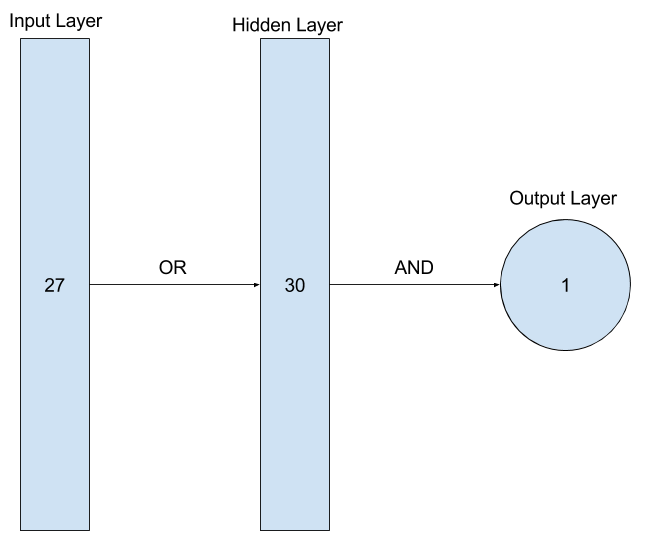
\includegraphics[width=\textwidth]{Tic-Tac-Toe-Net.png}
		\caption{Network architecture for learning Tic-Tac-Toe}
		\label{fig:tic-tac-toe-net}
	\end{minipage}
	\hfill
\end{figure}



\begin{table}[H]
	\begin{center}
		\begin{tabular}{| c | c | c | c | c |}
			\hline
			\textbf{} & \textbf{Net Error Rate} & \textbf{Net Error Rate CI} & \textbf{Rule Error Rate} & \textbf{Rule Error Rate CI 95\%}\\
			\hline
			\hline
			\textbf{Training} & 0.0035 & (0.0035, 0.0035) & 0.0000 & (0.0000, 0.0000)\\
			\textbf{Testing} & 0.0015 & (0.0015, 0.0015) & 0.0259 & (0.0104, 0.0451)\\
			\hline
		\end{tabular}
	\end{center}
	\caption{Results of experiments with Logical Neural Networks on the Tic Tac Toe problem}
	\label{tab:tic-tac-toe-lnn-peformance-results}
\end{table}

If instead ANDs are used as the hidden neurons and ORs for the outputs then the LNN is able to achieve statistically equivalent performance to the architecture in Figure \ref{fig:tic-tac-toe-net}. Table \ref{tab:tic-tac-toe-lnn-peformance-results-and-or} shows the results from these experiments.

\begin{table}[H]
	\begin{center}
		\begin{tabular}{| c | c | c | c | c |}
			\hline
			\textbf{} & \textbf{Net Error Rate} & \textbf{Net Error Rate CI} & \textbf{Rule Error Rate} & \textbf{Rule Error Rate CI 95\%}\\
			\hline
			\hline
			\textbf{Training} & 0.0035 & (0.0035, 0.0035) & 0.0000 & (0.0000, 0.0000)\\
			\textbf{Testing} & 0.0015 & (0.0015, 0.0015) & 0.0038 & (0.0, 0.0139)\\
			\hline
		\end{tabular}
	\end{center}
	\caption{Results of experiments with Logical Neural Networks on the Tic Tac Toe problem on a AND - OR Network}
	\label{tab:tic-tac-toe-lnn-peformance-results-and-or}
\end{table}

These experiments provide strong evidence against the conjecture stating that ANDs are not effective for extracting low level features.

\subsubsection{Evaluation of LNN Rules}
Figure \ref{fig:tic-tac-toe-rule-example} shows a rule taken at random from the AND OR network. This rule is saying that if the middle column contains all X's then X has won. There is redundancy in these rules as a cell can only be occupied by either an X, O or nothing.

\begin{figure}[H]
	\centering
	\begin{minipage}[t]{0.3\textwidth}
		\vspace{0px}
		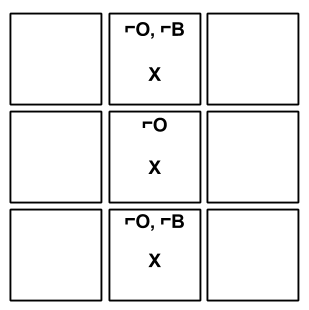
\includegraphics[width=\textwidth]{TicTacToe-RuleExample.png}
		\caption{A pictorial example of a rule extracted from the AND OR network}
		\label{fig:tic-tac-toe-rule-example}
	\end{minipage}
	\hspace{1cm}
	\begin{minipage}[t]{0.6\textwidth}
		\vspace{0px}
		A future goal might be to implement a way to build in mutual exclusivity of attributes into the network, this could result in further simplification of rules.\\

		The rule extraction algorithm given in Figure \ref{alg:rule-extraction} is an electic algorithm. This category describes algorithms that examine the network by inspecting each neuron but extract rules which represent the network as a whole \cite{tickle1998truth}. The algorithm is not portable as it can only be applied to networks with the LNN architecture.\\

	Finally what is the quality of the rules extracted from LNN? This is measured by the Accuracy, Fedelity, Consistency and Comprehensibility \cite{andrews1995survey}.
	\end{minipage}
	\hfill
\end{figure}

\begin{enumerate}
	\item \textbf{Accurate:} As demonstrated experimentally the extracted rules are able to generalise well when presented with unseen examples.
	\item \textbf{Fedelity:} The experiments show that the rules perform very similar to the network they where extracted from as both have a similar performance on the testing set.
	\item \textbf{Consistency:} These rule sets are consistent, shown by the low error rate when the neural network is trained from a number of different initial conditions.
	\item \textbf{Comprehensibility:} The upper limit of the total number of rules is a function of the networks size. The OR AND model obtains a complex set of rules, with a total 35 of the clauses. Whereas the AND OR model only utilizes 11 clauses. The network structure also contributes to the comprehensibility of the rules. For instance each clause in the AND OR rules represent a situation where the rule set is true. Where as in the OR AND model each clause must true.
\end{enumerate}

\subsection{Continuous Case}
Chapter \ref{C:investigation-of-lnfns} discusses three methods for intepreting Logical Normal Form Networks which can also be applied to the generalised LNN archetchure. Extracting a continous rule set would be to large to put in a report or intepret given MNIST has 784 features. For this reason Influence and Partial Influence models will be constructed and presented as images.

LNNs with no hidden layer can be intepreted easily by showing pictorial representations of Indluence models. Interpreting Multi Layer LNNs will be achieved by constructing Partial Influence models and then displaying pictorial representations of the most important features that contribute to the classification of an example as the digit 1. Multi-Layer perceptron networks will be visulised by constructing a heat map of the weights.

\subsubsection{No Hidden Layer Networks}

\paragraph{Sigmoid Network}
In the depictions of weights from a sigmoid network. The blue/red represents the negative/positive weights. The neuron which is representative of the classification as 0 does resemble the digit it is suppose to detect. The others do not appear to have any obvious relation to their digits.

\begin{figure}[H]
	\captionsetup{labelformat=empty}
	\centering
	\begin{minipage}[b]{0.19\textwidth}
		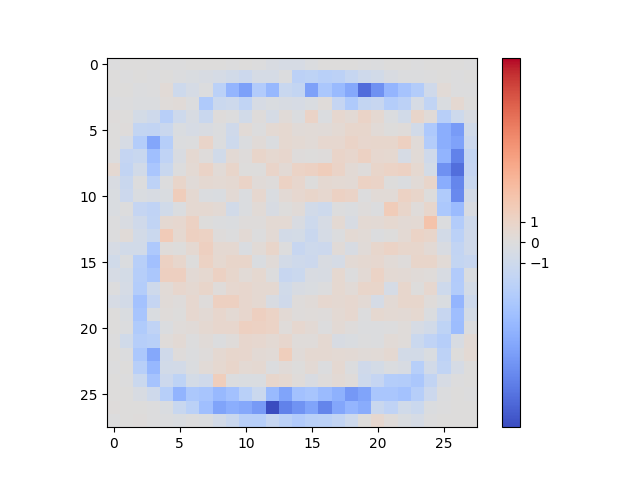
\includegraphics[width=\textwidth]{Sigmoid(NO-Hidden)/Layer0-Neuron-0.png}
		\caption{Digit 0}
	\end{minipage}
	\begin{minipage}[b]{0.19\textwidth}
		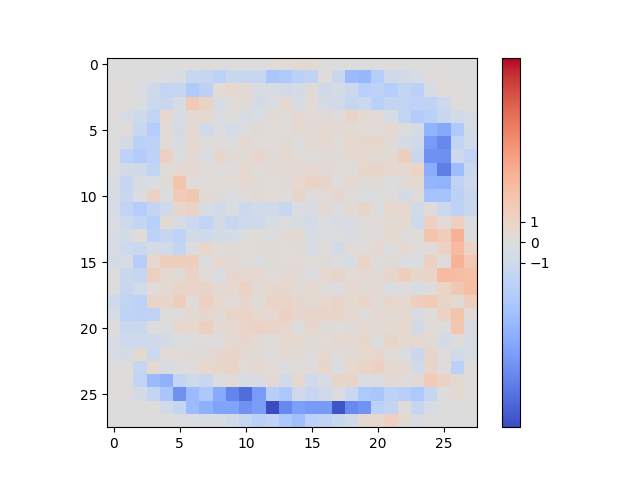
\includegraphics[width=\textwidth]{Sigmoid(NO-Hidden)/Layer0-Neuron-2.png}
		\caption{Digit 2}
	\end{minipage}
	\begin{minipage}[b]{0.19\textwidth}
		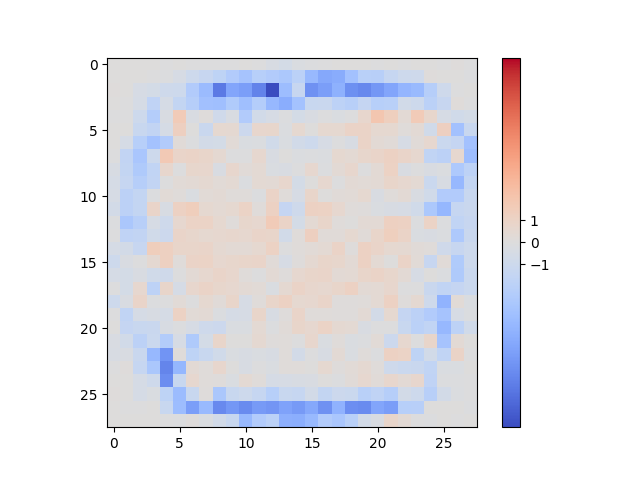
\includegraphics[width=\textwidth]{Sigmoid(NO-Hidden)/Layer0-Neuron-4.png}
		\caption{Digit 4}
	\end{minipage}
	\begin{minipage}[b]{0.19\textwidth}
		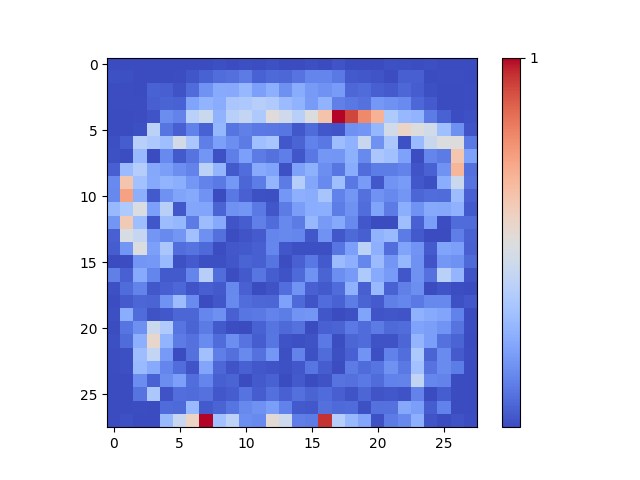
\includegraphics[width=\textwidth]{Sigmoid(NO-Hidden)/Layer0-Neuron-7.png}
		\caption{Digit 7}
	\end{minipage}
	\begin{minipage}[b]{0.19\textwidth}
		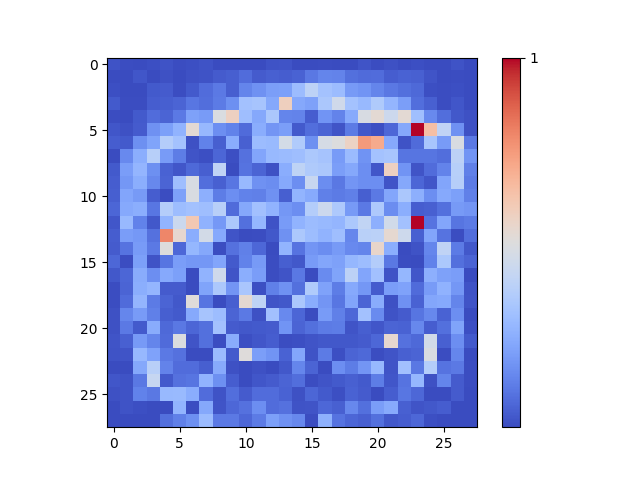
\includegraphics[width=\textwidth]{Sigmoid(NO-Hidden)/Layer0-Neuron-9.png}
		\caption{Digit 9}
	\end{minipage}
	\hfill
	\caption{Figures representing the output neurons of a sigmoid neural network with no hidden layers}
\end{figure}


\paragraph{AND Network Old Architecture (With and With Out LSM)}
The images in Figure \ref{fig:and-net-old-archetchure-interp} represent how relevant each input feature is towards a positive classification of the digits 0, 2, 4, 7 and 9. The top and bottom rows represents the relevance for an AND architecture with and without LSM retrospectively. The darker pixels represent more relevant features, where white is completely irrelevant.\\

The network without an LSM is using the pixels which occur in all representations of each digit. Whereas the network with an LSM is using the average filling to achieve its classifications. Both models are interpretable as it is possible to understand the logic used in their decision making. Each of the models describe the problem in a different way, each uncovering distinct information. The model without an LSM shows describes what is common between every drawing of that digit. The model with an LSM describes which parts of each digit vary the most/least. The benefit of the model with an LSM is that the pictorial representations appear to look more like the the digits which they classify. However the model without an LSM has a sparser representation so the model is dependent on less information.

\begin{figure}[H]
	%\captionsetup{labelformat=empty}
	\centering
	\begin{minipage}[b]{0.19\textwidth}
		\captionsetup{labelformat=empty}
		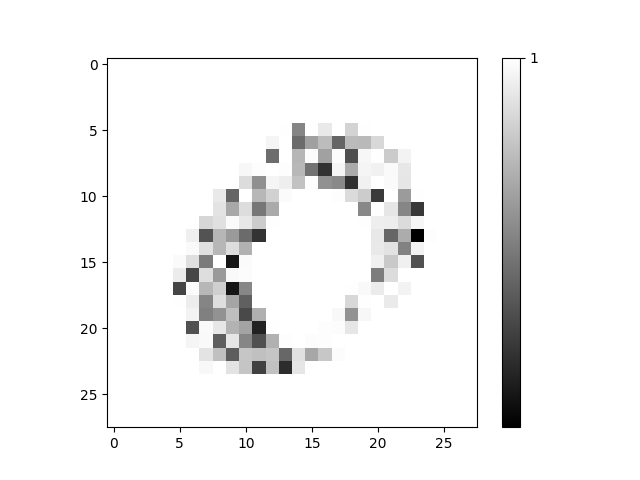
\includegraphics[width=\textwidth]{AND-OLD(LSM)/Layer0-Neuron-0.png}
		\caption{Digit 0}
	\end{minipage}
	\begin{minipage}[b]{0.19\textwidth}
		\captionsetup{labelformat=empty}
		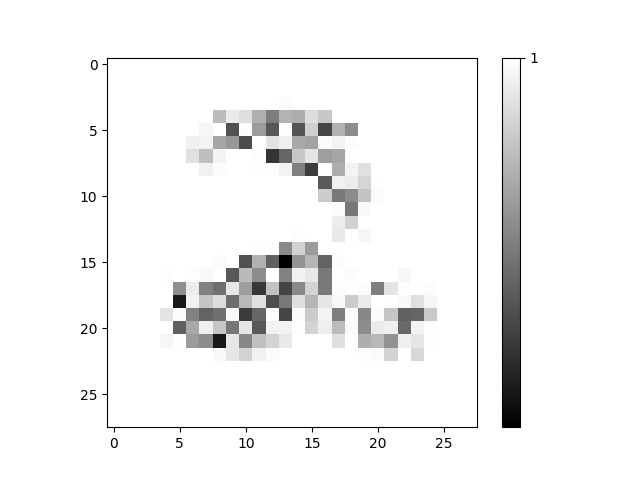
\includegraphics[width=\textwidth]{AND-OLD(LSM)/Layer0-Neuron-2.png}
		\caption{Digit 2}
	\end{minipage}
	\begin{minipage}[b]{0.19\textwidth}
		\captionsetup{labelformat=empty}
		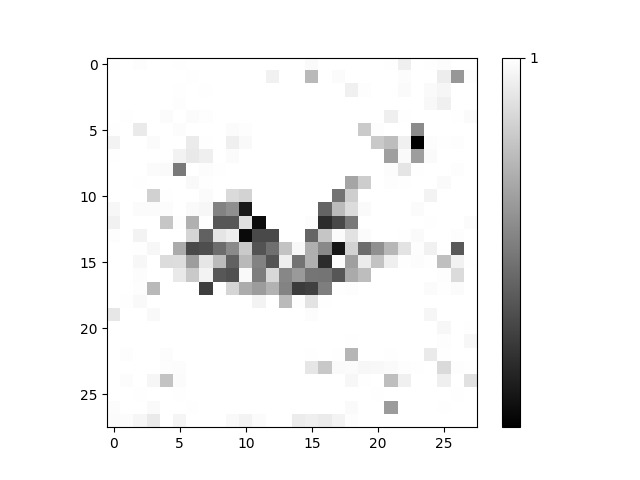
\includegraphics[width=\textwidth]{AND-OLD(LSM)/Layer0-Neuron-4.png}
		\caption{Digit 4}
	\end{minipage}
	\begin{minipage}[b]{0.19\textwidth}
		\captionsetup{labelformat=empty}
		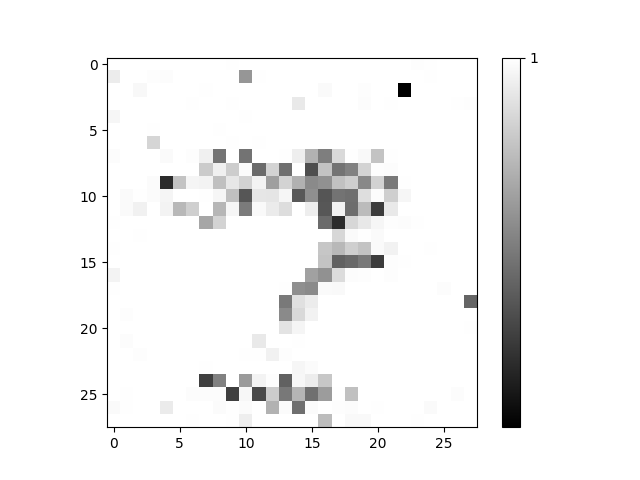
\includegraphics[width=\textwidth]{AND-OLD(LSM)/Layer0-Neuron-7.png}
		\caption{Digit 7}
	\end{minipage}
	\begin{minipage}[b]{0.19\textwidth}
		\captionsetup{labelformat=empty}
		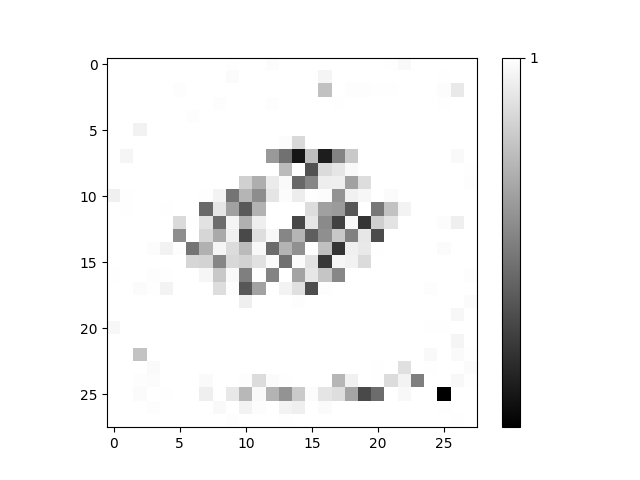
\includegraphics[width=\textwidth]{AND-OLD(LSM)/Layer0-Neuron-9.png}
		\caption{Digit 9}
	\end{minipage}
	\hfill
	\begin{minipage}[b]{0.19\textwidth}
		\captionsetup{labelformat=empty}
		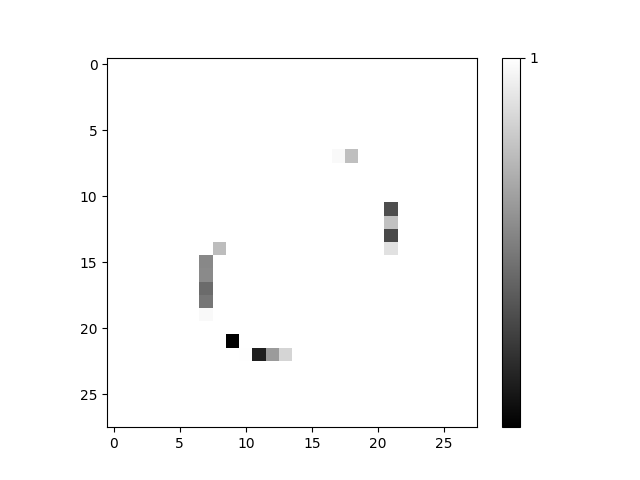
\includegraphics[width=\textwidth]{AND-OLD(NO-LSM)/Layer0-Neuron-0.png}
		\caption{Digit 0}
	\end{minipage}
	\begin{minipage}[b]{0.19\textwidth}
		\captionsetup{labelformat=empty}
		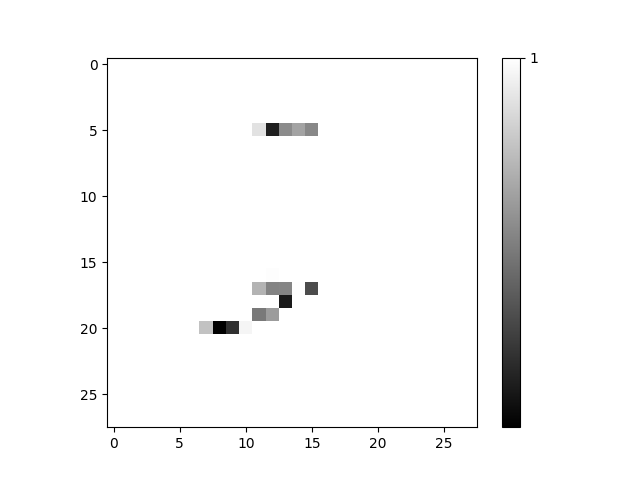
\includegraphics[width=\textwidth]{AND-OLD(NO-LSM)/Layer0-Neuron-2.png}
		\caption{Digit 2}
	\end{minipage}
	\begin{minipage}[b]{0.19\textwidth}
		\captionsetup{labelformat=empty}
		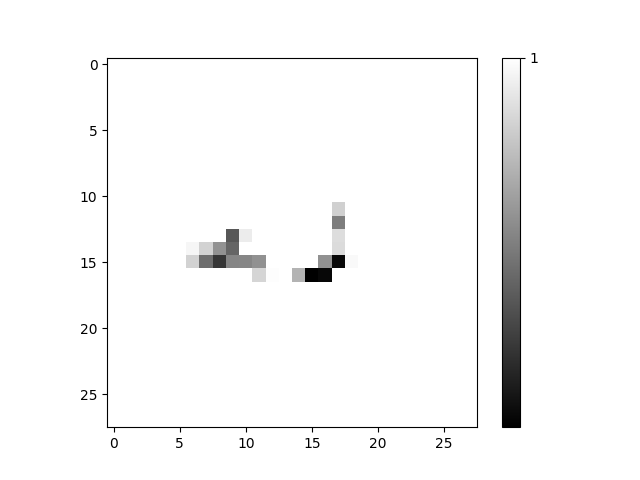
\includegraphics[width=\textwidth]{AND-OLD(NO-LSM)/Layer0-Neuron-4.png}
		\caption{Digit 4}
	\end{minipage}
	\begin{minipage}[b]{0.19\textwidth}
		\captionsetup{labelformat=empty}
		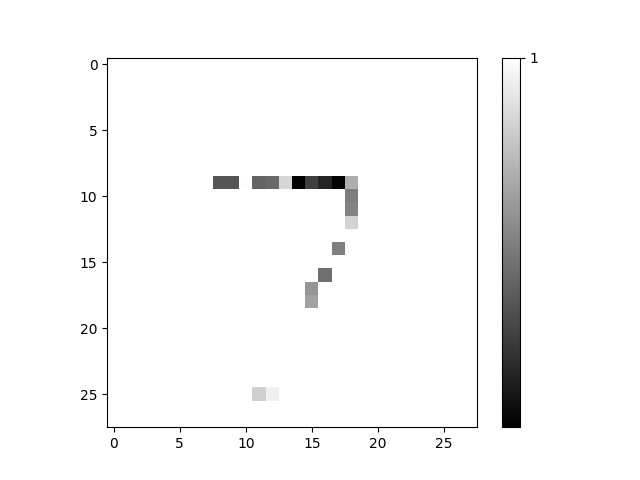
\includegraphics[width=\textwidth]{AND-OLD(NO-LSM)/Layer0-Neuron-7.png}
		\caption{Digit 7}
	\end{minipage}
	\begin{minipage}[b]{0.19\textwidth}
		\captionsetup{labelformat=empty}
		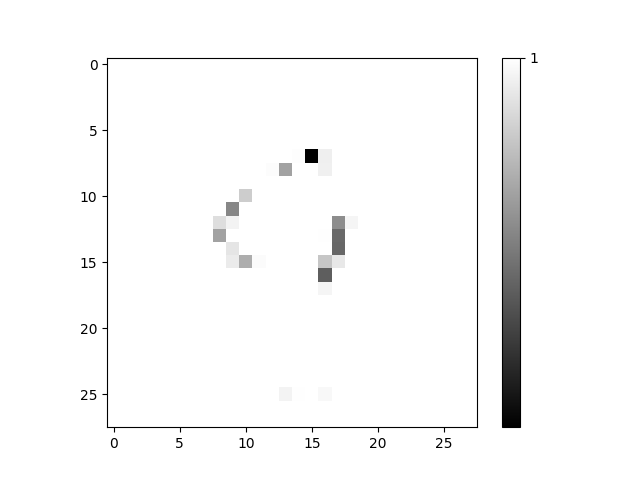
\includegraphics[width=\textwidth]{AND-OLD(NO-LSM)/Layer0-Neuron-9.png}
		\caption{Digit 9}
	\end{minipage}
	\hfill
	\caption{Figures representing the weighted connections between the inputs and outputs in an AND network with the old archetchure. Top row is with an LSM and bottom row is with out an LSM}
	\label{fig:and-net-old-archetchure-interp}
\end{figure}

\paragraph{AND Network (With LSM)}
The model here is an AND network running on the new archtchure (which considers the NOTs of inputs) with an LSM. The new archetchure means that each input feature can positively contribute to a classification or negatively contribute (i.e. if its present then the classification is less likely). Figure \ref{fig:and-net-new-archetchure-with-lsm-interp} shows the how relevent each input feature is with regards to a positive or negative classification for the digits 0, 2, 4, 7 and 9. The top row of images represent positively weighted inputs and the bottom row represents the negatively weighted inputs.\\

The inputs which are positively weighted are the pixels that occur in many of the representations of the digit. Negatively weighted inputs represent the border of the digit, if pixels on this border are present then the neuron is less likely to be active. Using the classification of 0 as an example, the network does not like pixels in the middle as the centre of a zero should be empty. The outer circle represents the border of the average 0, if these pixels are present then its less likely to be a zero as most instances of a 0 do not have pixels present there.

\begin{figure}[H]
	%\captionsetup{labelformat=empty}
	\centering
	\begin{minipage}[b]{0.19\textwidth}
		\captionsetup{labelformat=empty}
		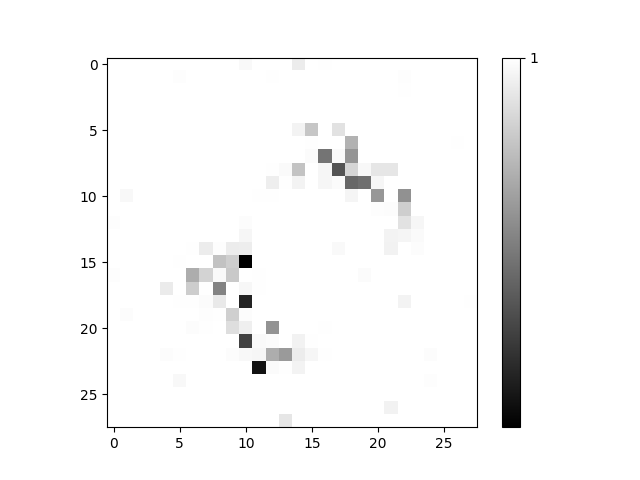
\includegraphics[width=\textwidth]{AND(LSM)/Positive/Layer0-Neuron-0.png}
		\caption{Digit 0}
	\end{minipage}
	\begin{minipage}[b]{0.19\textwidth}
		\captionsetup{labelformat=empty}
		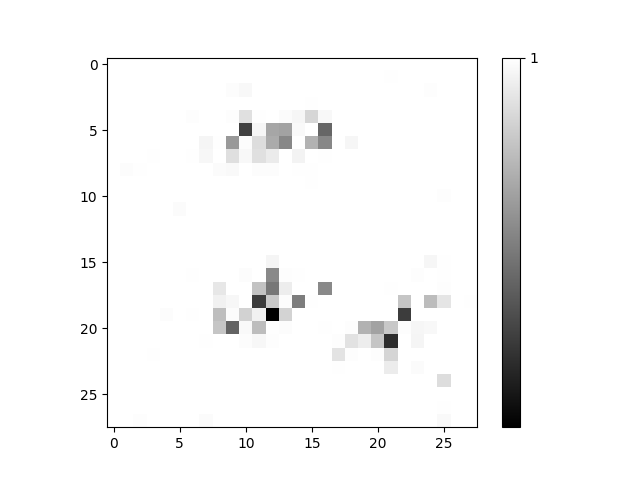
\includegraphics[width=\textwidth]{AND(LSM)/Positive/Layer0-Neuron-2.png}
		\caption{Digit 2}
	\end{minipage}
	\begin{minipage}[b]{0.19\textwidth}
		\captionsetup{labelformat=empty}
		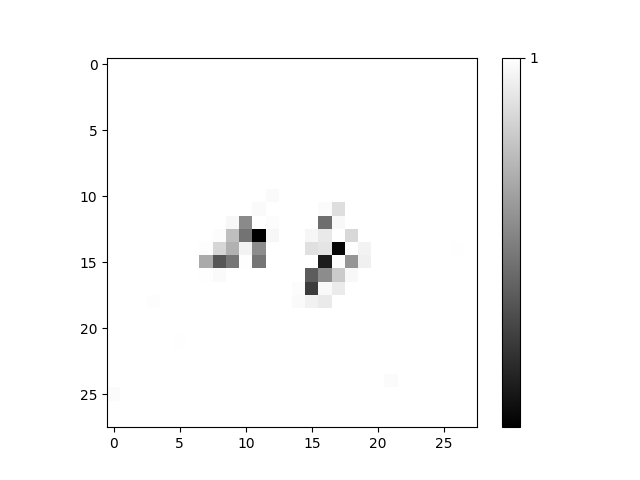
\includegraphics[width=\textwidth]{AND(LSM)/Positive/Layer0-Neuron-4.png}
		\caption{Digit 4}
	\end{minipage}
	\begin{minipage}[b]{0.19\textwidth}
		\captionsetup{labelformat=empty}
		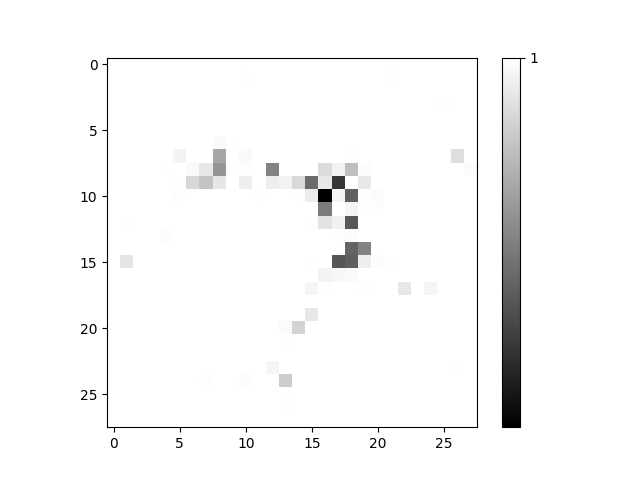
\includegraphics[width=\textwidth]{AND(LSM)/Positive/Layer0-Neuron-7.png}
		\caption{Digit 7}
	\end{minipage}
	\begin{minipage}[b]{0.19\textwidth}
		\captionsetup{labelformat=empty}
		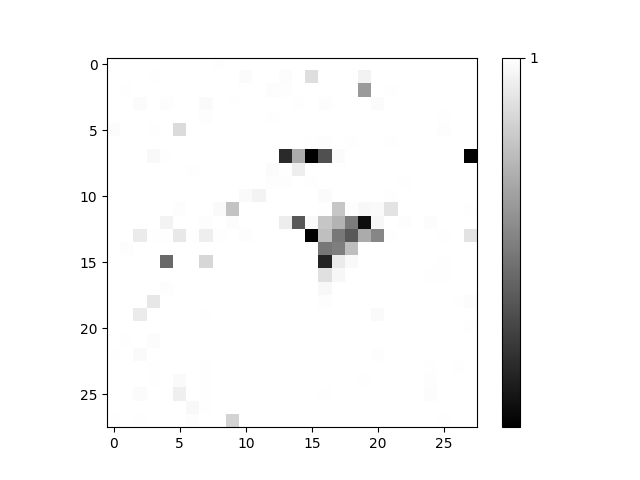
\includegraphics[width=\textwidth]{AND(LSM)/Positive/Layer0-Neuron-9.png}
		\caption{Digit 9}
	\end{minipage}
	\hfill
	\begin{minipage}[b]{0.19\textwidth}
		\captionsetup{labelformat=empty}
		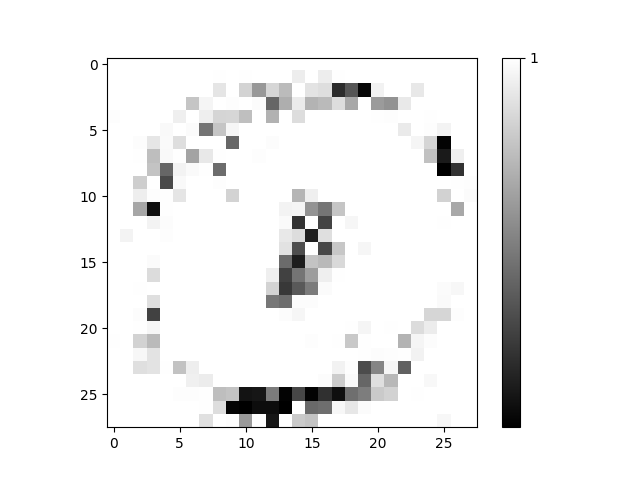
\includegraphics[width=\textwidth]{AND(LSM)/Negative/Layer0-Neuron-0.png}
		\caption{Not Digit 0}
	\end{minipage}
	\begin{minipage}[b]{0.19\textwidth}
		\captionsetup{labelformat=empty}
		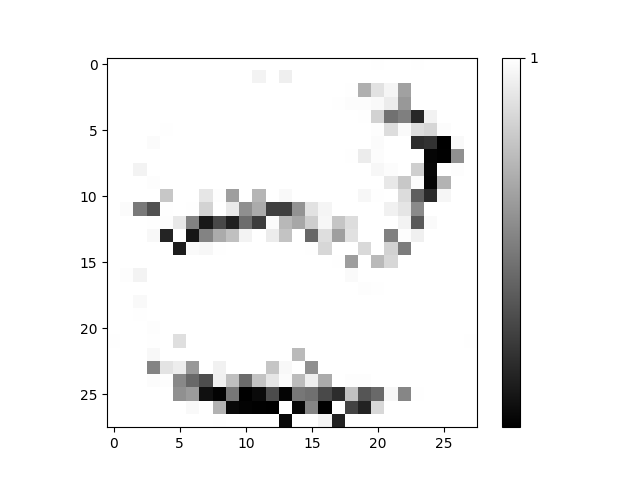
\includegraphics[width=\textwidth]{AND(LSM)/Negative/Layer0-Neuron-2.png}
		\caption{Not Digit 2}
	\end{minipage}
	\begin{minipage}[b]{0.19\textwidth}
		\captionsetup{labelformat=empty}
		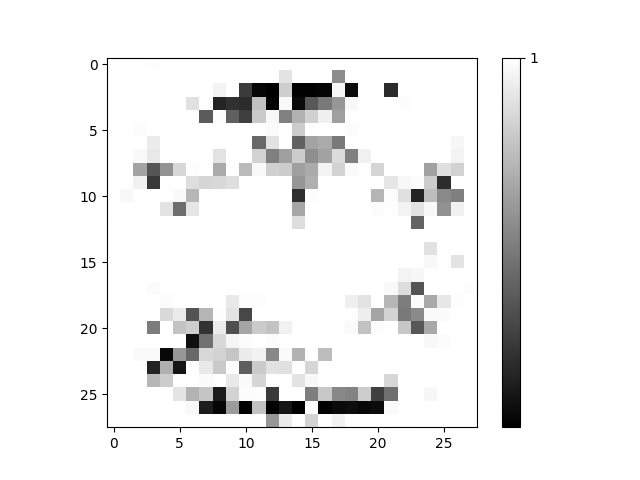
\includegraphics[width=\textwidth]{AND(LSM)/Negative/Layer0-Neuron-4.png}
		\caption{Not Digit 4}
	\end{minipage}
	\begin{minipage}[b]{0.19\textwidth}
		\captionsetup{labelformat=empty}
		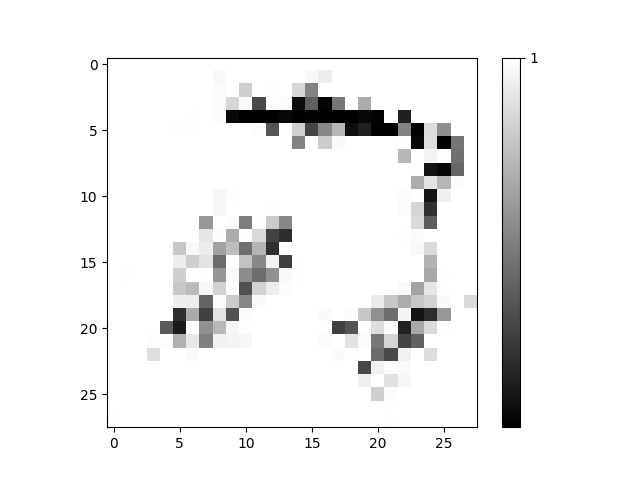
\includegraphics[width=\textwidth]{AND(LSM)/Negative/Layer0-Neuron-7.png}
		\caption{Not Digit 7}
	\end{minipage}
	\begin{minipage}[b]{0.19\textwidth}
		\captionsetup{labelformat=empty}
		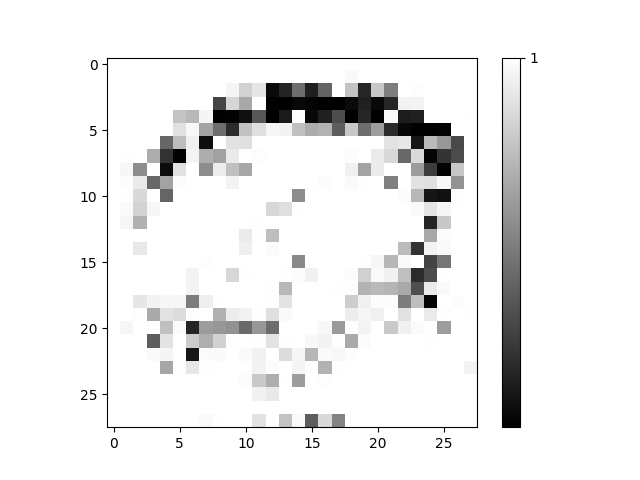
\includegraphics[width=\textwidth]{AND(LSM)/Negative/Layer0-Neuron-9.png}
		\caption{Not Digit 9}
	\end{minipage}
	\hfill
	\caption{Figures representing the weighted connections between the inputs and outputs for an AND network with an LSM. The top and bottom rows represent the positive/negative contributions retrospectively.}
	\label{fig:and-net-new-archetchure-with-lsm-interp}
\end{figure}

\paragraph{AND Network (With out LSM)}
Figure \ref{fig:and-net-new-archetchure-with-out-lsm-interp} shows the positive/negative contributions to classification of the digits 0, 2, 4, 7 and 9. These features display the same patterns as the AND model with an LSM (Figure \ref{fig:and-net-new-archetchure-with-lsm-interp}) however the representations here are less noisy and have harder boundaries.

\begin{figure}[H]
	%\captionsetup{labelformat=empty}
	\centering
	\begin{minipage}[b]{0.19\textwidth}
		\captionsetup{labelformat=empty}
		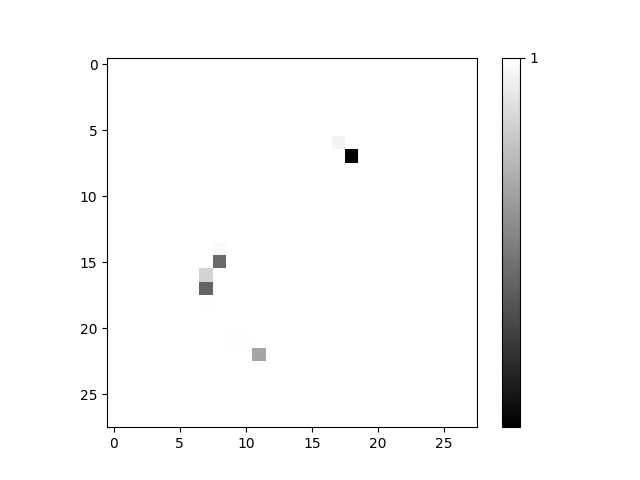
\includegraphics[width=\textwidth]{AND(NO-LSM)/Positive/Layer0-Neuron-0.png}
		\caption{Digit 0}
		\label{fig:cnf-descrete-generalizatiion}
	\end{minipage}
	\begin{minipage}[b]{0.19\textwidth}
		\captionsetup{labelformat=empty}
		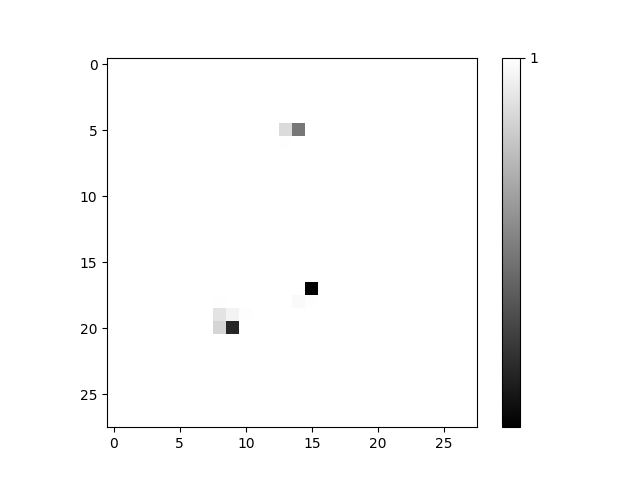
\includegraphics[width=\textwidth]{AND(NO-LSM)/Positive/Layer0-Neuron-2.png}
		\caption{Digit 2}
		\label{fig:cnf-descrete-generalizatiion}
	\end{minipage}
	\begin{minipage}[b]{0.19\textwidth}
		\captionsetup{labelformat=empty}
		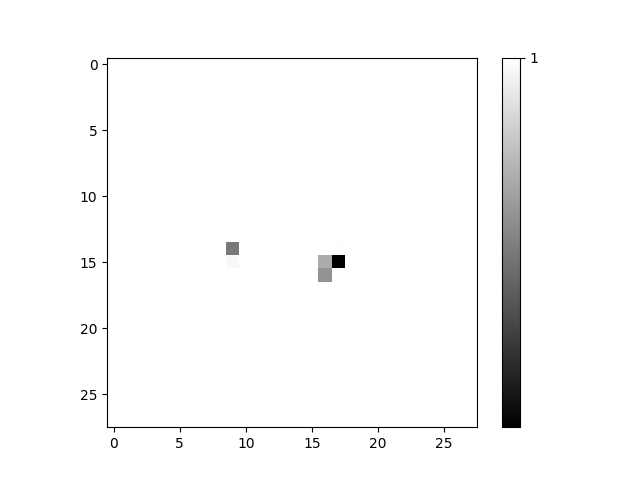
\includegraphics[width=\textwidth]{AND(NO-LSM)/Positive/Layer0-Neuron-4.png}
		\caption{Digit 4}
		\label{fig:cnf-descrete-generalizatiion}
	\end{minipage}
	\begin{minipage}[b]{0.19\textwidth}
		\captionsetup{labelformat=empty}
		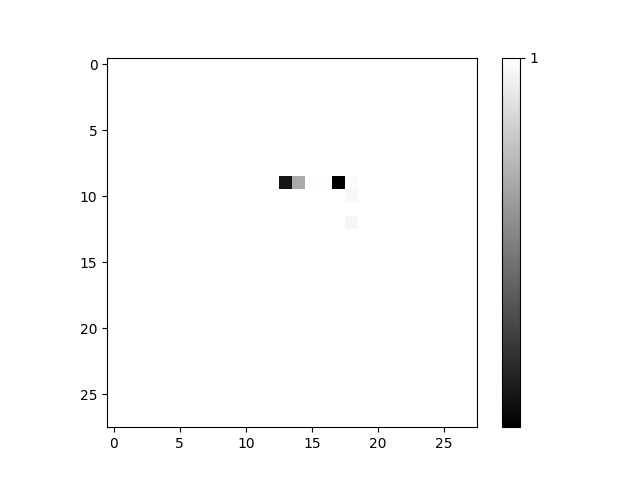
\includegraphics[width=\textwidth]{AND(NO-LSM)/Positive/Layer0-Neuron-7.png}
		\caption{Digit 7}
		\label{fig:cnf-descrete-generalizatiion}
	\end{minipage}
	\begin{minipage}[b]{0.19\textwidth}
		\captionsetup{labelformat=empty}
		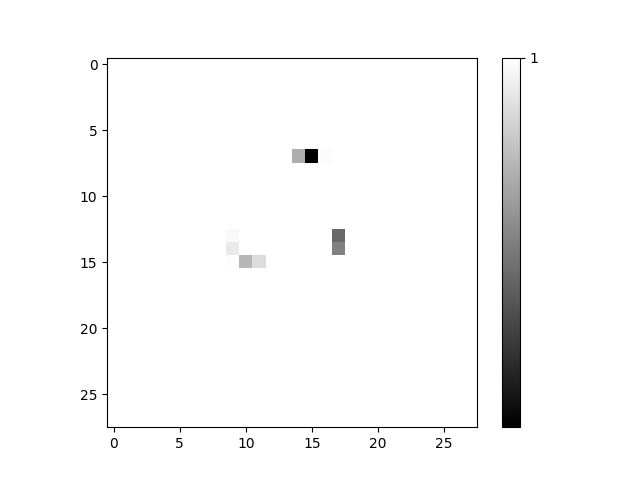
\includegraphics[width=\textwidth]{AND(NO-LSM)/Positive/Layer0-Neuron-9.png}
		\caption{Digit 9}
		\label{fig:cnf-descrete-generalizatiion}
	\end{minipage}
	\begin{minipage}[b]{0.19\textwidth}
		\captionsetup{labelformat=empty}
		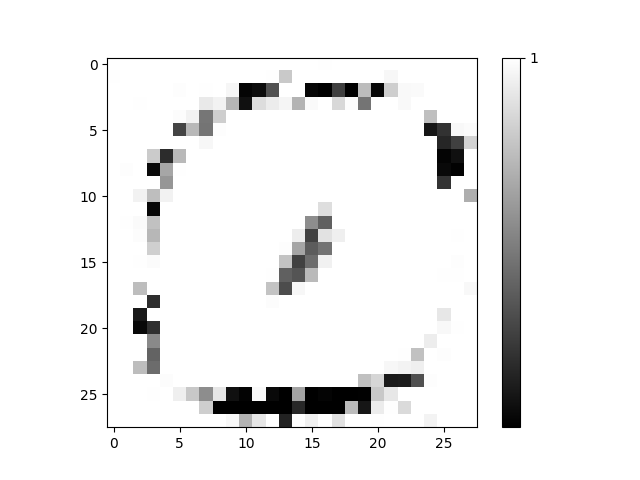
\includegraphics[width=\textwidth]{AND(NO-LSM)/Negative/Layer0-Neuron-0.png}
		\caption{Not Digit 0}
		\label{fig:cnf-descrete-generalizatiion}
	\end{minipage}
	\begin{minipage}[b]{0.19\textwidth}
		\captionsetup{labelformat=empty}
		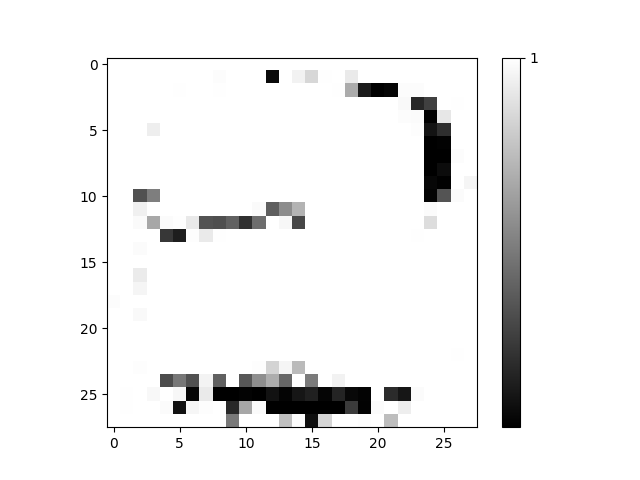
\includegraphics[width=\textwidth]{AND(NO-LSM)/Negative/Layer0-Neuron-2.png}
		\caption{Not Digit 2}
		\label{fig:cnf-descrete-generalizatiion}
	\end{minipage}
	\begin{minipage}[b]{0.19\textwidth}
		\captionsetup{labelformat=empty}
		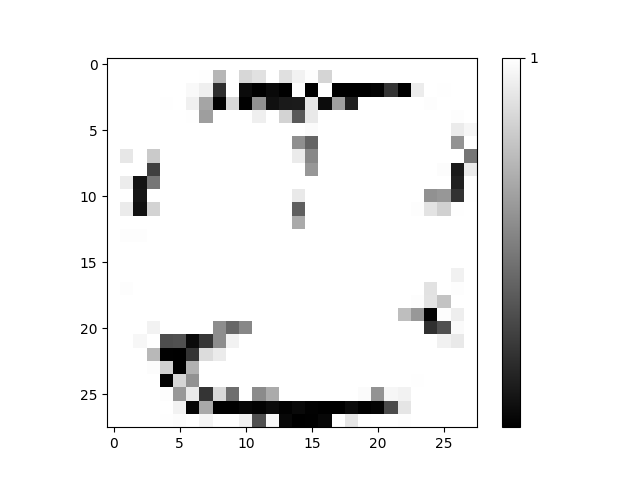
\includegraphics[width=\textwidth]{AND(NO-LSM)/Negative/Layer0-Neuron-4.png}
		\caption{Not Digit 4}
		\label{fig:cnf-descrete-generalizatiion}
	\end{minipage}
	\begin{minipage}[b]{0.19\textwidth}
		\captionsetup{labelformat=empty}
		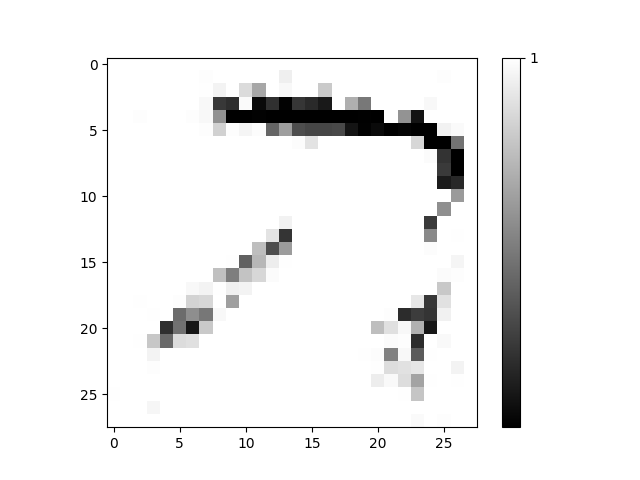
\includegraphics[width=\textwidth]{AND(NO-LSM)/Negative/Layer0-Neuron-7.png}
		\caption{Not Digit 7}
		\label{fig:cnf-descrete-generalizatiion}
	\end{minipage}
	\begin{minipage}[b]{0.19\textwidth}
		\captionsetup{labelformat=empty}
		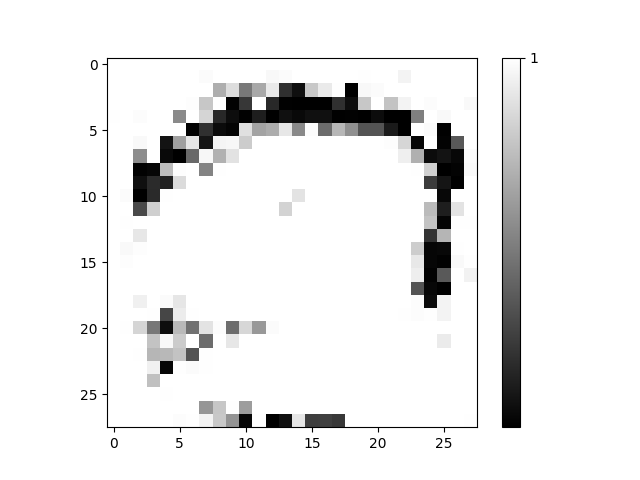
\includegraphics[width=\textwidth]{AND(NO-LSM)/Negative/Layer0-Neuron-9.png}
		\caption{Not Digit 9}
		\label{fig:cnf-descrete-generalizatiion}
	\end{minipage}
	\label{fig:and-net-new-archetchure-with-out-lsm-interp}
	\caption{The top/bottom rows of images represent the positively/negatively weighted input features retrospectively}
	\hfill
\end{figure}

\paragraph{Conclusion of Intepretability for LNNs with No Hidden Layer}
The logical Softmax introduces more noise into the weights but does not diminish the intepretability of the system. Using the new structure (i.e. adding nots of inputs) appears to change the means of which the LNN classifies the digits. Without NOTs the network positively weight the pixels which make-up the filling of the digits. On the other hand when the nots are added the network negatively weights pixels sitting just outside the border of the average digit.\\

These experiments provide evidence towards Logical Neural Networks being more interpretable than MLPNs. While it is possible to observe some of the MLPNs decision making process, the LNN is clearer and simpler leading to a more interpretable model.

\subsubsection{Single Hidden Layer Networks}
To intepret these multi layer networks Partial Influence models will be constructed and pictorial representations of the most important features that contrubute to classification as a one will be displayed.

\paragraph{Sigmoid Network}
	The features in Figure \ref{fig:sigmoid-hidden-layer-features-like} positively contribute to the classification as a 1. These do not appear to have any clear relation to the digit 1. The features in Figure \ref{fig:sigmoid-hidden-layer-features-dont-like} again appear to not have any relation ship with the digit 1.

	\begin{figure}[H]
		\centering
		\begin{minipage}[b]{0.19\textwidth}
			\captionsetup{labelformat=empty}
			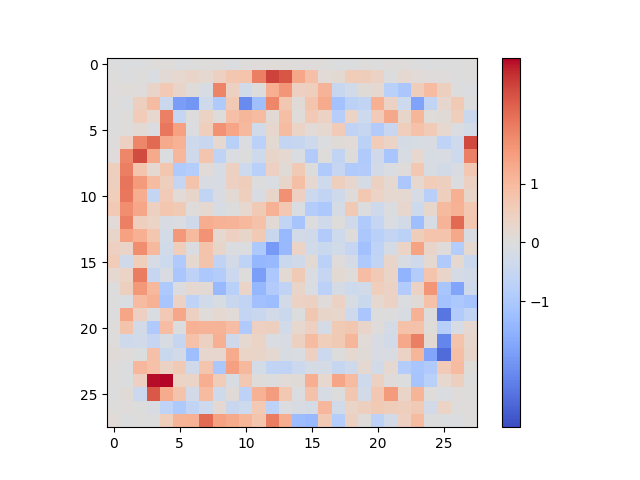
\includegraphics[width=\textwidth]{Sigmoid(Hidden-Layer)/Like/Layer0-Neuron-11.png}
			%\caption{Digit 0}
			\label{}
		\end{minipage}
		\begin{minipage}[b]{0.19\textwidth}
			\captionsetup{labelformat=empty}
			\includegraphics[width=\textwidth]{Sigmoid(Hidden-Layer)/Like/Layer0-Neuron-27.png}
			%\caption{Digit 0}
			\label{}
		\end{minipage}
		\begin{minipage}[b]{0.19\textwidth}
			\captionsetup{labelformat=empty}
			\includegraphics[width=\textwidth]{Sigmoid(Hidden-Layer)/Like/Layer0-Neuron-29.png}
			%\caption{Digit 0}
			\label{}
		\end{minipage}
		\caption{Features that positively contribute to the classification as a 1.}
		\label{fig:sigmoid-hidden-layer-features-like}
		\hfill
	\end{figure}

		\begin{figure}[H]
		\centering
		\begin{minipage}[b]{0.19\textwidth}
			\captionsetup{labelformat=empty}
			\includegraphics[width=\textwidth]{Sigmoid(Hidden-Layer)/DontLike/Layer0-Neuron-0.png}
			%\caption{Digit 0}
			\label{}
		\end{minipage}
		\begin{minipage}[b]{0.19\textwidth}
			\captionsetup{labelformat=empty}
			\includegraphics[width=\textwidth]{Sigmoid(Hidden-Layer)/DontLike/Layer0-Neuron-4.png}
			%\caption{Digit 0}
			\label{}
		\end{minipage}
		\caption{Features that negatively contribute to the classification of 1}
		\label{fig:sigmoid-hidden-layer-features-dont-like}
		\hfill
	\end{figure}

\begin{minipage}[t]{0.45\textwidth}
	\vspace{0px}

	
	\paragraph{OR $\rightarrow$ AND Network Old Structure (With Out LSM)}
	It is not immediately apparent how the features in Figure \ref{fig:or-and-net-old-with-out-lsm} make up the digit 1. \\
	
	Each hidden feature is an OR of its inputs, as such only one of the dark pixels needs to be active for the neuron to be on. The first and last could be the stem of a 1 where as the middle one contains a dark bar at the bottom which could be the base.

	\paragraph{OR $\rightarrow$ AND Network Old Structure (With LSM)}
	Figure \ref{fig:or-and-net-old-with-lsm} shows hidden features extracted from an OR AND Network. These features are not clearly representative of a 1. The weighting maps show that the features generally do not place a lot of emphasis on any particular inputs.

\end{minipage}
\hspace{0.1\textwidth}
\begin{minipage}[t]{0.45\textwidth}
	\vspace{0px}
	

	\begin{figure}[H]
		%\captionsetup{labelformat=empty}
		\centering
		\begin{minipage}[b]{0.33\textwidth}
			\captionsetup{labelformat=empty}
			\includegraphics[width=\textwidth]{OR-AND(OLD)(WO-LSM)(1)/Layer0-Neuron-5.png}
			%\caption{Digit 0}
			\label{}
		\end{minipage}
		\begin{minipage}[b]{0.33\textwidth}
			\captionsetup{labelformat=empty}
			\includegraphics[width=\textwidth]{OR-AND(OLD)(WO-LSM)(1)/Layer0-Neuron-15.png}
			%\caption{Digit 0}
			\label{}
		\end{minipage}
		\begin{minipage}[b]{0.33\textwidth}
			\captionsetup{labelformat=empty}
			\includegraphics[width=\textwidth]{OR-AND(OLD)(WO-LSM)(1)/Layer0-Neuron-23.png}
			%\caption{Digit 0}
			\label{}
		\end{minipage}
		\caption{Features positively contributing to classification as a 1 for the OR $\rightarrow$ AND Network}
		\label{fig:or-and-net-old-with-out-lsm}
		\hfill
	\end{figure}
\end{minipage}


\begin{figure}[H]
	%\captionsetup{labelformat=empty}
	\centering
	\begin{minipage}[b]{0.19\textwidth}
		\captionsetup{labelformat=empty}
		\includegraphics[width=\textwidth]{OR-AND(OLD)(W-LSM)(1)/Layer0-Neuron-0.png}
		%\caption{Digit 0}
		\label{}
	\end{minipage}
	\begin{minipage}[b]{0.19\textwidth}
		\captionsetup{labelformat=empty}
		\includegraphics[width=\textwidth]{OR-AND(OLD)(W-LSM)(1)/Layer0-Neuron-2.png}
		%\caption{Digit 0}
		\label{}
	\end{minipage}
	\begin{minipage}[b]{0.19\textwidth}
		\captionsetup{labelformat=empty}
		\includegraphics[width=\textwidth]{OR-AND(OLD)(W-LSM)(1)/Layer0-Neuron-6.png}
		%\caption{Digit 0}
		\label{}
	\end{minipage}
	\begin{minipage}[b]{0.19\textwidth}
		\captionsetup{labelformat=empty}
	\includegraphics[width=\textwidth]{OR-AND(OLD)(W-LSM)(1)/Layer0-Neuron-7.png}
	%\caption{Digit 0}
	\label{}
	\end{minipage}
	\begin{minipage}[b]{0.19\textwidth}
		\captionsetup{labelformat=empty}
		\includegraphics[width=\textwidth]{OR-AND(OLD)(W-LSM)(1)/Layer0-Neuron-10.png}
		%\caption{Digit 0}
		\label{}
	\end{minipage}
	\begin{minipage}[b]{0.19\textwidth}
		\captionsetup{labelformat=empty}
		\includegraphics[width=\textwidth]{OR-AND(OLD)(W-LSM)(1)/Layer0-Neuron-14.png}
		%\caption{Digit 0}
		\label{}
	\end{minipage}
		\begin{minipage}[b]{0.19\textwidth}
		\captionsetup{labelformat=empty}
		\includegraphics[width=\textwidth]{OR-AND(OLD)(W-LSM)(1)/Layer0-Neuron-20.png}
		%\caption{Digit 0}
		\label{}
	\end{minipage}
	\begin{minipage}[b]{0.19\textwidth}
		\captionsetup{labelformat=empty}
		\includegraphics[width=\textwidth]{OR-AND(OLD)(W-LSM)(1)/Layer0-Neuron-29.png}
		%\caption{Digit 0}
		\label{}
	\end{minipage}
	\caption{Features positively contributing to the classification of 1 for the OR $\rightarrow$ AND Network Old Structure (With LSM)}
	\label{fig:or-and-net-old-with-lsm}
	
	\hfill
\end{figure}


\begin{minipage}[t]{0.3\textwidth}
	\vspace{0px}
\paragraph{OR $\rightarrow$ AND Network (With Out LSM)}
The images in Figure \ref{fig:or-and-net-without-lsm-pos} represent the hidden 
features which positively contribute to the classification of an example as the digit 1. The top and bottom rows correspond to the input features that positively/negatively contribute to each neurons activation. It is not immediately obvious what the features shown in Figure \ref{fig:or-and-net-without-lsm-pos} represent.\\
\end{minipage}
\hspace{0.1\textwidth}
\begin{minipage}[t]{0.6\textwidth}
	\vspace{0px}
	\begin{figure}[H]
		%\captionsetup{labelformat=empty}
		\centering
		\begin{minipage}[b]{0.24\textwidth}
			\captionsetup{labelformat=empty}
			\includegraphics[width=\textwidth]{OR-AND(WO-LSM)(1)/Like/True/Layer0-Neuron-0.png}
			%\caption{Digit 0}
			\label{}
		\end{minipage}
		\begin{minipage}[b]{0.24\textwidth}
			\captionsetup{labelformat=empty}
			\includegraphics[width=\textwidth]{OR-AND(WO-LSM)(1)/Like/True/Layer0-Neuron-3.png}
			%\caption{Digit 0}
			\label{}
		\end{minipage}
		\begin{minipage}[b]{0.24\textwidth}
			\captionsetup{labelformat=empty}
			\includegraphics[width=\textwidth]{OR-AND(WO-LSM)(1)/Like/True/Layer0-Neuron-10.png}
			%\caption{Digit 0}
			\label{}
		\end{minipage}
		\begin{minipage}[b]{0.24\textwidth}
			\captionsetup{labelformat=empty}
			\includegraphics[width=\textwidth]{OR-AND(WO-LSM)(1)/Like/True/Layer0-Neuron-15.png}
			%\caption{Digit 0}
			\label{}
		\end{minipage}
		
		\medskip
		
		\begin{minipage}[b]{0.24\textwidth}
			\captionsetup{labelformat=empty}
			\includegraphics[width=\textwidth]{OR-AND(WO-LSM)(1)/Like/False/Layer0-Neuron-0.png}
			%\caption{Digit 0}
			\label{}
		\end{minipage}
		\begin{minipage}[b]{0.24\textwidth}
			\captionsetup{labelformat=empty}
			\includegraphics[width=\textwidth]{OR-AND(WO-LSM)(1)/Like/False/Layer0-Neuron-3.png}
			%\caption{Digit 0}
			\label{}
		\end{minipage}
		\begin{minipage}[b]{0.24\textwidth}
			\captionsetup{labelformat=empty}
			\includegraphics[width=\textwidth]{OR-AND(WO-LSM)(1)/Like/False/Layer0-Neuron-10.png}
			%\caption{Digit 0}
			\label{}
		\end{minipage}
		\begin{minipage}[b]{0.24\textwidth}
			\captionsetup{labelformat=empty}
			\includegraphics[width=\textwidth]{OR-AND(WO-LSM)(1)/Like/False/Layer0-Neuron-15.png}
			%\caption{Digit 0}
			\label{}
		\end{minipage}
		\caption{Features positively contributing to classification as a 1 for OR $\rightarrow$ AND Network (With Out LSM)}
		\label{fig:or-and-net-without-lsm-pos}
		\hfill
	\end{figure}
\end{minipage}

\begin{minipage}[t]{0.5\textwidth}
	\vspace{0cm}
Figure \ref{fig:or-and-net-without-lsm-neg} shows the single feature which if present then the classification is less likely to be the digit 1. This feature appears to be highly active if the pixels lying outside an area which looks like the average 1 shape.\\

While this model is difficult to interpret it does provide more information than previous OR AND models using the old LNN architecture.
		
\paragraph{OR $\rightarrow$ AND (With LSM)} Figure \ref{fig:or-and-with-lsm-pos} show the positive features for an OR AND model with an LSM. 
The features extracted from this network do not appear to correspond to a 1, not in a way which is immediately interpretable. 
\end{minipage}
\hspace{0.1\textwidth}
\begin{minipage}[t]{0.4\textwidth}
	\vspace{0px}
	%\captionsetup{labelformat=empty}
	\begin{figure}[H]
		\centering
		\begin{minipage}[b]{0.45\textwidth}
			\captionsetup{labelformat=empty}
			\includegraphics[width=\textwidth]{OR-AND(WO-LSM)(1)/DontLike/True/Layer0-Neuron-28.png}
			%\caption{Digit 0}
			\label{}
		\end{minipage}
	
		\medskip
	
		\begin{minipage}[b]{0.45\textwidth}
			\captionsetup{labelformat=empty}
			\includegraphics[width=\textwidth]{OR-AND(WO-LSM)(1)/DontLike/False/Layer0-Neuron-28.png}
			%\caption{Digit 0}
			\label{}
		\end{minipage}
		\caption{Features contributing to classification not being 1 for OR $\rightarrow$ AND Network (With Out LSM)}
		\label{fig:or-and-net-without-lsm-neg}
		\hfill
	\end{figure}
\end{minipage}

\begin{minipage}[t]{0.45\textwidth}
	\vspace{0.2px}
	The presence of the features represented in Figure \ref{fig:or-and-with-lsm-neg} mean the classification is less likely to be a 1. These features do not appear to relate to the digit 1, but rather pixels that would not usually occur in the digit 1.\\
		
	\begin{figure}[H]	
		%\captionsetup{labelformat=empty}
		\centering
		\begin{minipage}[b]{0.32\textwidth}
			\captionsetup{labelformat=empty}
			\includegraphics[width=\textwidth]{OR-AND(W-LSM)(1)/DontLike/True/Layer0-Neuron-2.png}
			%\caption{Digit 0}
			\label{}
		\end{minipage}
		\begin{minipage}[b]{0.32\textwidth}
			\captionsetup{labelformat=empty}
			\includegraphics[width=\textwidth]{OR-AND(W-LSM)(1)/DontLike/True/Layer0-Neuron-9.png}
			%\caption{Digit 0}
			\label{}
		\end{minipage}
		\begin{minipage}[b]{0.32\textwidth}
			\captionsetup{labelformat=empty}
			\includegraphics[width=\textwidth]{OR-AND(W-LSM)(1)/DontLike/True/Layer0-Neuron-28.png}
			%\caption{Digit 0}
			\label{}
		\end{minipage}
			
		\medskip
			
		\begin{minipage}[b]{0.32\textwidth}
			\captionsetup{labelformat=empty}
			\includegraphics[width=\textwidth]{OR-AND(W-LSM)(1)/DontLike/False/Layer0-Neuron-2.png}
			%\caption{Digit 0}
			\label{}
		\end{minipage}
		\begin{minipage}[b]{0.32\textwidth}
			\captionsetup{labelformat=empty}
			\includegraphics[width=\textwidth]{OR-AND(W-LSM)(1)/DontLike/False/Layer0-Neuron-9.png}
			%\caption{Digit 0}
			\label{}
		\end{minipage}
		\begin{minipage}[b]{0.32\textwidth}
			\captionsetup{labelformat=empty}
			\includegraphics[width=\textwidth]{OR-AND(W-LSM)(1)/DontLike/False/Layer0-Neuron-28.png}
			%\caption{Digit 0}
			\label{}
		\end{minipage}
			\caption{Features contributing to the classification not being 1 for OR $\rightarrow$ AND (With LSM)}
			\label{fig:or-and-with-lsm-neg}
			\hfill
	\end{figure}
	
	\paragraph{AND $\rightarrow$ OR Model (With Out LSM)}
	Figure \ref{fig:and-or-with-out-lsm-lnn-features-pos} shows the single feature which positively contributes to the classification as the digit 1. This feature has learnt to positively identify the stem of a 1 and negatively identify .\\
		
	This network has a small number of features associated with each classification. In terms of the classifying the digit 1 there is only 1 hidden features. This feature appears to classify a 1 by positively liking the stem of a 1 and disliking the anything outside the average 1.\\
		
	\paragraph{AND $\rightarrow$ OR Model (With LSM)}
	Similarly to the AND OR Model with out the LSM this model appears to positively like inputs on the stem of a 1 and dislike any pixel outside the average border of a 1. These features are shown in Figure \ref{fig:and-or-lnn-with-lsm-like}
\end{minipage}
\hspace{0.1\textwidth}
\begin{minipage}[t]{0.45\textwidth}
	\vspace{0cm}
	\begin{figure}[H]
		\begin{minipage}[b]{0.5\textwidth}
			\captionsetup{labelformat=empty}
			\includegraphics[width=\textwidth]{OR-AND(W-LSM)(1)/Like/True/Layer0-Neuron-18.png}
			%\caption{Digit 0}
			\label{}
		\end{minipage}
		\begin{minipage}[b]{0.45\textwidth}
			\captionsetup{labelformat=empty}
			\includegraphics[width=\textwidth]{OR-AND(W-LSM)(1)/Like/True/Layer0-Neuron-19.png}
			%\caption{Digit 0}
			\label{}
		\end{minipage}
		
		\medskip
		
		\begin{minipage}[b]{0.45\textwidth}
			\captionsetup{labelformat=empty}
			\includegraphics[width=\textwidth]{OR-AND(W-LSM)(1)/Like/False/Layer0-Neuron-18.png}
			%\caption{Digit 0}
			\label{}
		\end{minipage}
		\begin{minipage}[b]{0.45\textwidth}
			\captionsetup{labelformat=empty}
			\includegraphics[width=\textwidth]{OR-AND(W-LSM)(1)/Like/False/Layer0-Neuron-19.png}
			%\caption{Digit 0}
			\label{}
		\end{minipage}
		\caption{Features positively contributing to the classification being 1 for OR $\rightarrow$ AND (With LSM)}
		\label{fig:or-and-with-lsm-pos}
	\end{figure}

	\begin{figure}[H]
			\centering
		\begin{minipage}[b]{0.5\textwidth}
			\captionsetup{labelformat=empty}
			\includegraphics[width=\textwidth]{AND-OR(WO-LSM)(1)/Like/True/Layer0-Neuron-3.png}
			%\caption{Digit 0}
			\label{}
		\end{minipage}
		
		\medskip
		
		\begin{minipage}[b]{0.5\textwidth}
			\captionsetup{labelformat=empty}
			\includegraphics[width=\textwidth]{AND-OR(WO-LSM)(1)/Like/False/Layer0-Neuron-3.png}
			%\caption{Digit 0}
			\label{}
		\end{minipage}
		\caption{Features positively contributing to classification as 1 for AND $\rightarrow$ OR Model (With Out LSM)}
		\label{fig:and-or-with-out-lsm-lnn-features-pos}
	\end{figure}
\end{minipage}


\begin{minipage}[t]{0.45\textwidth}
	\vspace{0px}
	\paragraph{Conclusion of Intepretability for LNNs with No Hidden Layer}
	The results of the experiments show that in the context of multi layer adding an LSM introduces more noise into the feature maps. And similarly to before the sigmoid weights do not appear to relate to digit 1 in any meaningful way.
\end{minipage}
\hspace{0.1\textwidth}
\begin{minipage}[t]{0.45\textwidth}
	\vspace{0px}
		%\captionsetup{labelformat=empty}
	\begin{figure}[H]
		\centering
		\begin{minipage}[b]{0.5\textwidth}
			\captionsetup{labelformat=empty}
			\includegraphics[width=\textwidth]{AND-OR(W-LSM)(1)/Like/True/Layer0-Neuron-9.png}
			%\caption{Digit 0}
			\label{}
		\end{minipage}
		
		\medskip
		
		\begin{minipage}[b]{0.5\textwidth}
			\captionsetup{labelformat=empty}
			\includegraphics[width=\textwidth]{AND-OR(W-LSM)(1)/Like/False/Layer0-Neuron-9.png}
			%\caption{Digit 0}
			\label{}
		\end{minipage}
		\caption{Features contributing to classification not being 1 for AND $\rightarrow$ OR Model (With Out LSM)}
		\label{fig:and-or-lnn-with-lsm-like}
		\hfill
	\end{figure}
	
\end{minipage}


\subsection{Results of Intepretability Experiments}
From the above experiments and discussions the following conclusions can be made

\begin{enumerate}
	\item \textit{Rules Extracted are Intepretable:} The Tic-Tac-Toe problem experiments showed that the rules extracted from LNNs where interpretable.
	\item \textit{Adding Nots Improves Intepretability:} Using the new structure with nots allows the network to place a greater emphasis on the presence or absence of various pixels. Without the Nots not many of inputs are of great importance, rather many have a relatively small relevance.
	\item \textit{Adding an Logical Soft Max does not hinder the intepretability (on the new architecture):} By comparing the two different network architectures with and without an LSM it is possible to see that the intepretability is not directly effected and the features representing the classification of the digit 1 are not significantly changed.
	\item \textit{Intepretability of Network is Heavily Dependent on Structure:} As shown through the previous examples the OR $\rightarrow$ AND networks harder to interpret than the AND $\rightarrow$ OR architecture.
\end{enumerate}

\section{Comparason Between LNNs and Exsisting Methods}
\subsection{Comparison between LNN Intepretability and LIME}
The aim of LIME is to build trust in the model by explaining how a specific predictions are arrived at. LIME is also model agnostic, so it is a highly portable algorithm.  In comparason, LNN intepretability comes down to directly identifying what input features contribute to each output neuron being active. Figure \ref{} shows the LIME algorythm applied to three different ANNs, two LNNs and one MLPN. Each image shows what features are important in classifiying the example as a 1.

\begin{figure}[H]
	\begin{minipage}[b]{0.33\textwidth}
		\captionsetup{labelformat=empty}
		\includegraphics[width=\textwidth]{LIME/LNN-(AND).png}
		%\caption{Digit 0}
		\label{}
	\end{minipage}
	\begin{minipage}[b]{0.33\textwidth}
		\captionsetup{labelformat=empty}
		\includegraphics[width=\textwidth]{LIME/LNN-(OR-AND-AND).png}
		%\caption{Digit 0}
		\label{}
	\end{minipage}
	\begin{minipage}[b]{0.33\textwidth}
		\captionsetup{labelformat=empty}
		\includegraphics[width=\textwidth]{LIME/MLPN.png}
		%\caption{Digit 0}
		\label{}
	\end{minipage}
	\caption{Features contributing to classification not being 1 for AND $\rightarrow$ OR Model (With Out LSM)}
	\label{fig:and-or-lnn-with-lsm-like}
\end{figure}

The LIME filters out the features which have a low importance. Figure \ref{fig:and-or-lnn-with-lsm-like} says that for the three different classifiers the same features are most important to correctly classifiying this instance of a 1. 

\subsection{Comparason Between LNNs and Fuzzy Logic Networks}
The paper presenting Fuzzy Logic Networks (FLN) evaluates their peformance on a number of benchmark problems including the Vehicle \cite{Lichman:2013} dataset. The Vehicle problem concerns attempting to classify a given silhouette as one of four vehicles types. The data set consists of 18 features extracted from car silhoute images.\\

\begin{table}[H]
	\begin{center}
		\begin{tabular}{| c | c | c | c | c |}
			\hline
			\textbf{} & \textbf{Net Error Rate} & \textbf{Net Error Rate CI} & \textbf{Rule Error Rate} & \textbf{Rule Error Rate CI 95\%}\\
			\hline
			\hline
			\textbf{Training} & 0.101 & (0.079, 0.132) & 0.649 & (0.380, 0.762)\\
			\textbf{Testing} & 0.173 & (0.130, 0.224) & 0.648 & (0.398, 0.763)\\
			\hline
		\end{tabular}
	\end{center}
	\caption{Results of experiments with Logical Neural Networks on the Vehicle Problem using an OR $\rightarrow$ OR $\rightarrow$ AND network archetchure}
	\label{tab:vehicle-lnn-peformance}
\end{table}

Tabel \ref{tab:vehicle-lnn-peformance} show the error rates of OR $\rightarrow$ OR $\rightarrow$ AND LNN on the Vehicle problem. The LNN network achieved an average error rate of --\& on a testing set compared to 28.71\% error rate for the FLN. The difference between the LNN and rule error rates is stisticaly significant. While the rules extracted from an LNN peform worse than the network its self they have comparable peformance to rules taken from a FLN. An LNN rule set obtains 64.8\% average error rate on the test set where as the FLN rules achieve an average error rate of 67.8\%.\\

One advantage that the FLN has over LNNs is that the rule sets are more compact and thus are simpler to intepret. This experement would sugest that FLN is better than LNNs as the rule sets have similar peformance but FLN rules are simpler. Future work on LNNs might aim to implement an algorythm which can automatically simplyfy the extracted rules, this could lead to simpler expressions.

\section{Summary Of Logical Neural Network Evaluation}
Through the experiments carried out the following observations can be made. The new LNN structure (adding NOTs) results with a statistically significant increase in accuracy with some network architectures. The new LNN structure achieved statistically equivalent or better performance than the MLPN nets with an equivalent number of hidden neurons/layers. For any LNN (new structure or old) adding a Logical Softmax improved performance by a statistically significant margin. Any LNN (new or old structure) was more interpretable than the corresponding MLPN. These experiments have therefore shown that the LNN networks have statistically equivalent performance to MLPNs on the MNIST dataset. Evidence has also been provided in support of LNNs have a more interpretable model than MLPNs.\\

The LIME algorythm is more powerful than LNN Intepretability in the sense that it is model agnostic. On the other hand Intepreting LNNs provides a more complete picture of the models decison making process. Comparing LNNs and Fuzzy Logic Networks on the Vehicles problem showed that the LNN error rate was lower. However, ultimately a more interesting comparason is how the rule sets peform on a test set. Both LNN and FLN yield rules that obtain a comparable error rate the only difference between the two being FLN rules are simpler.

\chapter{Application to Auto Encoders} \label{C:lnn-application}
This chapter demonstrates the flexibility of the LNN architecture by applying them in the context of Auto Encoders. \\

Auto encoders \cite{baldi2012complex} \cite{hinton2006reducing} are a network architecture trained with unsupervised learning for a purpose of learning an encoding of the data. An application learning a new encoding is dimensionality reduction. The aim is to take the input to some reduced feature space and then from this feature space back to the original input with the smallest error. The case where there is one linear layer doing the encoding and decoding is called \textbf{Linear Autoencoder}. Logical Autoencoders are proposed (Definition \ref{def:logical-autoencoder}) as an alternative means to lower the dimensions of a dataset.

\begin{definition} \label{def:logical-autoencoder}
	A \textbf{Logical Autoencoder} is an Autoencoder where the encoder and decoder are LNNs
\end{definition}

Linear, Sigmoid and Logical Autoencoders will be compared. The network structure will be the same in all cases, only differing in the activations used. Experiments carried out will compress the MNIST feature space (784 dimensions) into 20. The accuracy and intepretability of the features will be explored. Each model was trained for 30 epochs

\paragraph{Result of Linear Autoencoder (LAE)}
A linear auto encoder obtained an MSE of 21.34 on the training and 21.25 on the test data. Figure \ref{fig:linear-autoencoder-features} shows a visualisation of some features learnt by the Linear Auto Encoder

\begin{figure}[H]
	%\captionsetup{labelformat=empty}
	\centering
	\begin{minipage}[b]{0.19\textwidth}
		\captionsetup{labelformat=empty}
		\includegraphics[width=\textwidth]{Linear-AE/Feature-3.png}
		%\caption{Digit 0}
		\label{}
	\end{minipage}
	\begin{minipage}[b]{0.19\textwidth}
		\captionsetup{labelformat=empty}
		\includegraphics[width=\textwidth]{Linear-AE/Feature-7.png}
		%\caption{Digit 0}
		\label{}
	\end{minipage}
	\begin{minipage}[b]{0.19\textwidth}
		\captionsetup{labelformat=empty}
		\includegraphics[width=\textwidth]{Linear-AE/Feature-11.png}
		%\caption{Digit 0}
		\label{}
	\end{minipage}
	\begin{minipage}[b]{0.19\textwidth}
		\captionsetup{labelformat=empty}
		\includegraphics[width=\textwidth]{Linear-AE/Feature-15.png}
		%\caption{Digit 0}
		\label{}
	\end{minipage}
	\begin{minipage}[b]{0.19\textwidth}
		\captionsetup{labelformat=empty}
		\includegraphics[width=\textwidth]{Linear-AE/Feature-18.png}
		%\caption{Digit 0}
		\label{}
	\end{minipage}
	
	\caption{Visualisations of 5 features learnt by the Linear Auto Encoder. The red colours correspond to positive weights and the blue to negative}
	\label{fig:linear-autoencoder-features}
	\hfill
\end{figure}

\paragraph{Result of Sigmoid Auto Encoder (SAE)}
A Sigmoid Autoencoder achieved an MSE of 14.43 on the training data and 14.25 on the testing data. Figure \ref{fig:sigmoid-autoencoder-features} show the visual representations of the features learnt.

\begin{figure}[H]
	%\captionsetup{labelformat=empty}
	\centering
	\begin{minipage}[b]{0.19\textwidth}
		\captionsetup{labelformat=empty}
		\includegraphics[width=\textwidth]{SAE(20LF)/Feature-0.png}
		%\caption{Digit 0}
		\label{}
	\end{minipage}
	\begin{minipage}[b]{0.19\textwidth}
		\captionsetup{labelformat=empty}
		\includegraphics[width=\textwidth]{SAE(20LF)/Feature-6.png}
		%\caption{Digit 0}
		\label{}
	\end{minipage}
	\begin{minipage}[b]{0.19\textwidth}
		\captionsetup{labelformat=empty}
		\includegraphics[width=\textwidth]{SAE(20LF)/Feature-10.png}
		%\caption{Digit 0}
		\label{}
	\end{minipage}
	\begin{minipage}[b]{0.19\textwidth}
		\captionsetup{labelformat=empty}
		\includegraphics[width=\textwidth]{SAE(20LF)/Feature-12.png}
		%\caption{Digit 0}
		\label{}
	\end{minipage}
	\begin{minipage}[b]{0.19\textwidth}
		\captionsetup{labelformat=empty}
		\includegraphics[width=\textwidth]{SAE(20LF)/Feature-15.png}
		%\caption{Digit 0}
		\label{}
	\end{minipage}
	\caption{Visualisations of 5 features learnt by the Sigmoid Auto Encoder. The red colours correspond to positive weights and the blue to negative}
	\label{fig:sigmoid-autoencoder-features}
	\hfill
\end{figure}

\paragraph{Result of Logical Auto Encoder (LoAE)}
A logical auto encoder, consisting of a single AND layer for both the encoder and decoder, was able to compress the feature space to 20 dimensions and achieve a Mean Square Error (MSE) of 20.55 on the training set and 20.22 on the testing set. Figure \ref{fig:logical-autoencoder-features} shows five features learnt by the AND-Logical Autoencoder. Each image in the top row represents the input features which positively contribute to the activation. The bottom row correspond to the inputs which negatively contribute to each activation. 

\begin{figure}[H]
	%\captionsetup{labelformat=empty}
	\centering
	\begin{minipage}[b]{0.19\textwidth}
		\captionsetup{labelformat=empty}
		\includegraphics[width=\textwidth]{LoAE(AND)(20LF)/True/Feature-0.png}
		%\caption{Digit 0}
		\label{}
	\end{minipage}
	\begin{minipage}[b]{0.19\textwidth}
		\captionsetup{labelformat=empty}
		\includegraphics[width=\textwidth]{LoAE(AND)(20LF)/True/Feature-4.png}
		%\caption{Digit 0}
		\label{}
	\end{minipage}
	\begin{minipage}[b]{0.19\textwidth}
		\captionsetup{labelformat=empty}
		\includegraphics[width=\textwidth]{LoAE(AND)(20LF)/True/Feature-10.png}
		%\caption{Digit 0}
		\label{}
	\end{minipage}
	\begin{minipage}[b]{0.19\textwidth}
		\captionsetup{labelformat=empty}
		\includegraphics[width=\textwidth]{LoAE(AND)(20LF)/True/Feature-12.png}
		%\caption{Digit 0}
		\label{}
	\end{minipage}
	\begin{minipage}[b]{0.19\textwidth}
		\captionsetup{labelformat=empty}
		\includegraphics[width=\textwidth]{LoAE(AND)(20LF)/True/Feature-17.png}
		%\caption{Digit 0}
		\label{}
	\end{minipage}
	
	\medskip
	
	\begin{minipage}[b]{0.19\textwidth}
		\captionsetup{labelformat=empty}
		\includegraphics[width=\textwidth]{LoAE(AND)(20LF)/False/Feature-0.png}
		%\caption{Digit 0}
		\label{}
	\end{minipage}
	\begin{minipage}[b]{0.19\textwidth}
		\captionsetup{labelformat=empty}
		\includegraphics[width=\textwidth]{LoAE(AND)(20LF)/False/Feature-4.png}
		%\caption{Digit 0}
		\label{}
	\end{minipage}
	\begin{minipage}[b]{0.19\textwidth}
		\captionsetup{labelformat=empty}
		\includegraphics[width=\textwidth]{LoAE(AND)(20LF)/False/Feature-10.png}
		%\caption{Digit 0}
		\label{}
	\end{minipage}
	\begin{minipage}[b]{0.19\textwidth}
		\captionsetup{labelformat=empty}
		\includegraphics[width=\textwidth]{LoAE(AND)(20LF)/False/Feature-12.png}
		%\caption{Digit 0}
		\label{}
	\end{minipage}
	\begin{minipage}[b]{0.19\textwidth}
		\captionsetup{labelformat=empty}
		\includegraphics[width=\textwidth]{LoAE(AND)(20LF)/False/Feature-17.png}
		%\caption{Digit 0}
		\label{}
	\end{minipage}
	\caption{Visualisations of 5 features learnt by the Logical Auto Encoder. Darker regions correspond to pixels which are relevant.}
	\label{fig:logical-autoencoder-features}
	\hfill
\end{figure}

\paragraph{Discussion}
While the results show that the Sigmoid Auto Encoder (AE) outperforms the Logical one this is an example of how Logical Neural Networks can be applied to different situations in Machine Learning where the goals are different from classification. Comparing Figures \ref{fig:linear-autoencoder-features} \& \ref{fig:sigmoid-autoencoder-features} \& \ref{fig:logical-autoencoder-features} show that the Logical Autoencoder takes a different approach to decomposing the MNIST dataset, where the Sigmoid and Linear took to be similar. Features learnt by the Logical AE are sparse and possible interpretable as each one can be viewed as a logical AND of the input features.
